\documentclass[letterpaper,12pt]{book}
\usepackage[margin=0.75in]{geometry}
\usepackage{moreverb}
\usepackage{float}
\usepackage{subfigure}
\usepackage{graphicx}
\usepackage{epstopdf}

% Define the \sourcelst command to create a floating listing of 
% a (separate) source file.
\newfloat{listing}{t}{lop}
\floatname{listing}{Listing}
\def\sourcelst#1#2{
\begin{listing}
\begin{tabular}{|@{\hspace{0.04\linewidth}}c@{\hspace{0.02\linewidth}}|}
\hline \\
\begin{minipage}{0.94\linewidth}
\small\listinginput{1}{#1}
\end{minipage}
\\ \\ \hline
\end{tabular}
\caption{[{\tt #1}]\ \ #2}
\label{lst:#1}
\end{listing}
}

\title{{\Huge The Vision Workbook:}\\A User's Guide to the\\NASA Vision Workbench v1.0}
\author{
Matthew D.~Hancher\\
Michael J.~Broxton\\
Laurence J.~Edwards\\
\\
Intelligent Systems Division\\
NASA Ames Research Center\\
\\
DRAFT}

\begin{document}
\maketitle
\chapter*{Acknowledgements}

Many people have contributed to making this first Vision Workbench
open-source release a reality.  Thanks to Terry Fong, Kalamanje
KrishnaKumar, and Dave Korsmeyer in the Intelligent Systems Division
at NASA Ames for supporting us in this research and allowing us to
pursue our crazy dreams.  Thanks to Larry Barone, Martha Del Alto,
Robin Orans, Diana Cox, and everyone else who helped us navigate the
NASA open source release process.  Thanks to Randy Sargent, Matt
Deans, Liam Pedersen, and the rest of the Intelligent Robotics Group
at Ames for lending their incredible expertise and being our guinea
pigs time and again.  Thanks to our interns---Kerri Cahoy, Ian Saxton,
Patrick Mihelich, Joey Gannon, and Aaron Rolett---for bringing many
exciting features of the Vision Workbench into being.  Finally, thanks
to all our users, past, present and future, for making software
development enjoyable and worthwhile.

Portions of this work were funded by the Mars Critical Data Products
Initiative, the Mars Exploration Technology Program, and the
Exploration Technology Development Program.

\tableofcontents
\chapter{Introduction}

This document is designed to be a gentle introduction to programming
with the NASA Vision Workbench, a C++ image processing and machine
vision library.  The Vision Workbench was developed through a joint
effort of the Intelligent Robotics Group (IRG) and the Adaptive
Control and Evolvable Systems Group (ACES) within the Intelligent
Systems Division at the NASA Ames Research Center in Moffett Field,
California.  It is distributed under the NASA Open Source Agreement
(NOSA) version 1.3, which has been certified by the Open Source
Initiative (OSI).  A copy of this agreement is included with every
distribution of the Vision Workbench in a file called {\tt COPYING}.

You can think of the Vision Workbench as a ``second-generation'' C/C++
image processing library.  It draws on the authors' experiences over
the past decade working with a number of ``first-generation''
libraries, such as OpenCV and VXL, as well as direct implementations
of image processing algorithms in C.  We have tried to select and
improve upon the best features of each of these approaches to image
processing, always with an eye toward our particular range of NASA
research applications.  The Vision Workbench has been used within NASA
for a wide range of image processing tasks, including alignment and
stitching of panoramic images, high-dynamic-range imaging, texture
analysis and recognition, lunar and planetary map generation, and the
production of 3D models from stereo image pairs.  A few examples of
image data that has been processed with the Vision Workbench are show
in Figure~\ref{fig:examples}.

\begin{figure}[p]
\centering
  \subfigure[]{\hbox{\hspace{0.25in}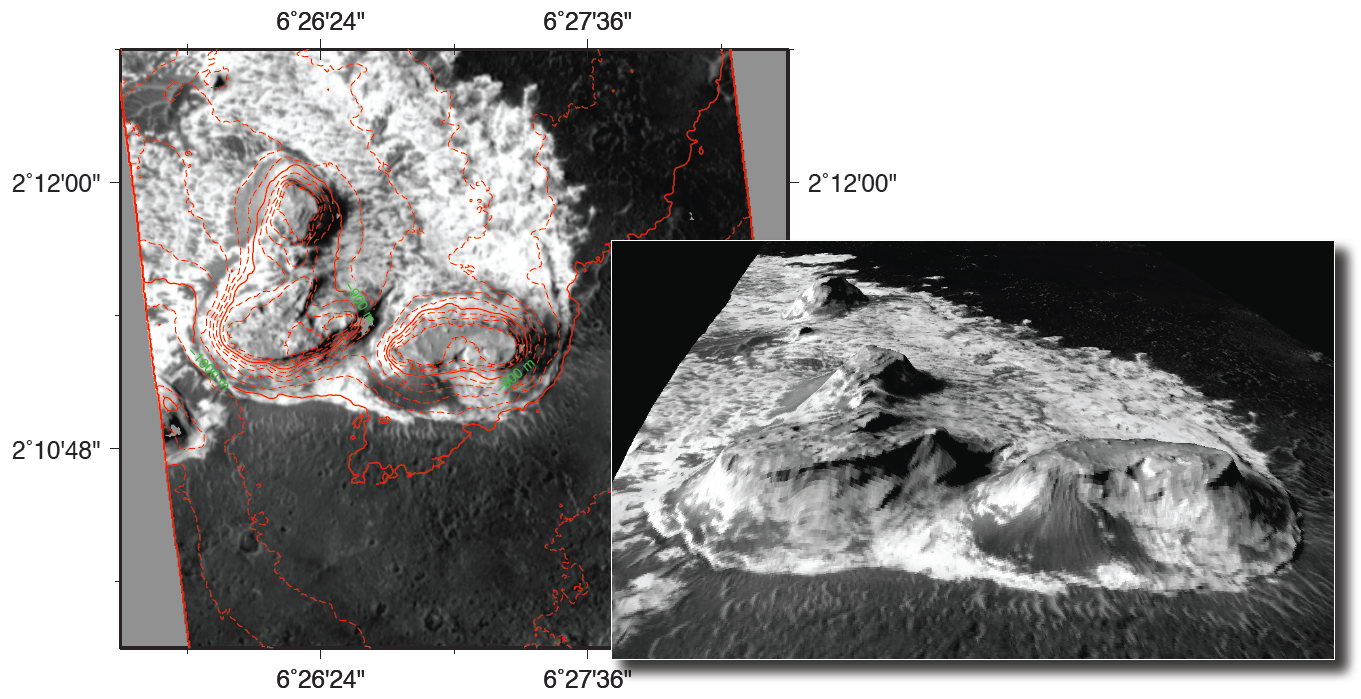
\includegraphics[width=5in]{images/mars_dem.png}\hspace{0.25in}\ \label{fig:examples.marsdem}}}
  \\
  \subfigure[]{\hbox{\hspace{0.25in}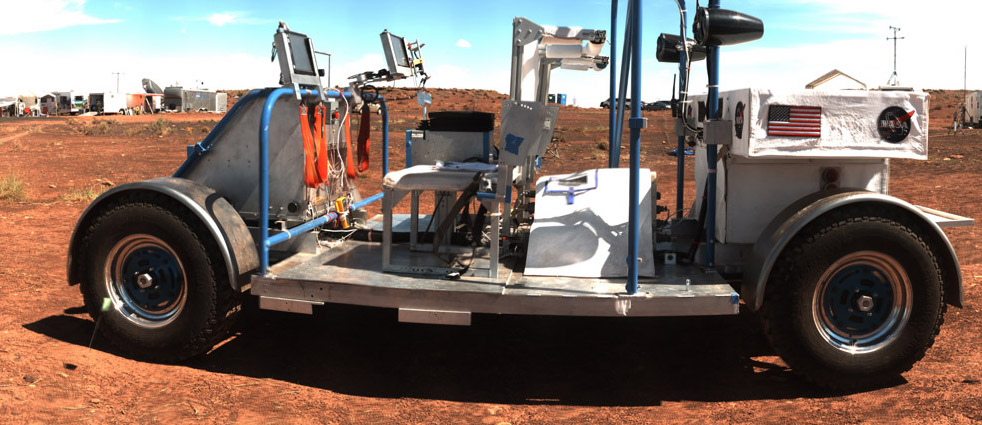
\includegraphics[width=2.75in]{images/scout_ldr.jpg}\hspace{0.25in}\ \label{fig:examples.scoutldr}}}
  \hfil
  \subfigure[]{\hbox{\hspace{0.25in}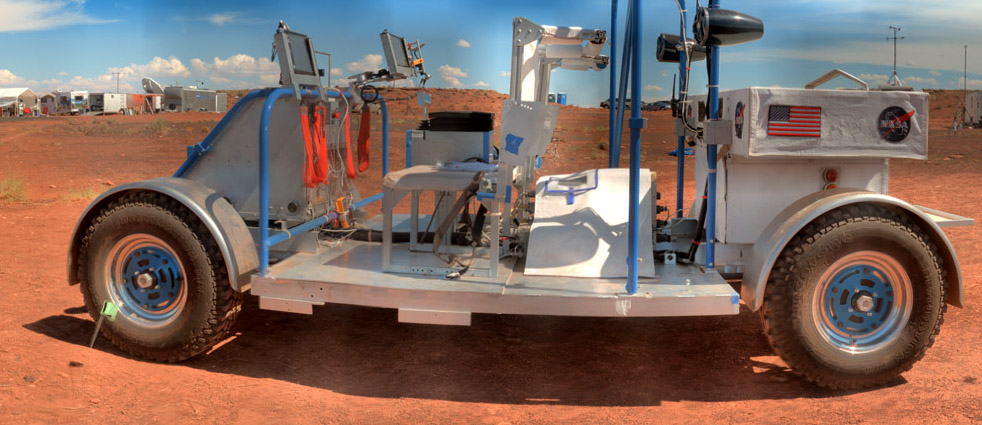
\includegraphics[width=2.75in]{images/scout_hdr.jpg}\hspace{0.25in}\ \label{fig:examples.scouthdr}}}
  \\
  \subfigure[]{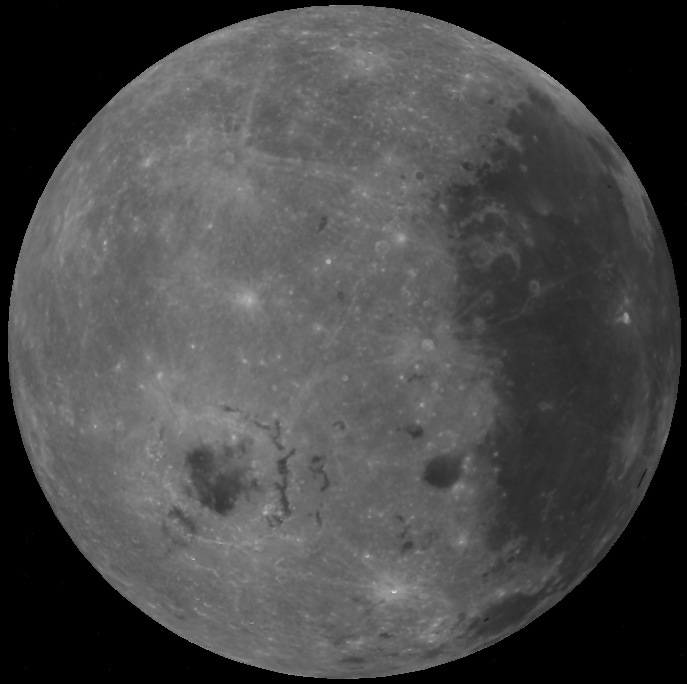
\includegraphics[width=2.5in]{images/moon_sphere.jpg}\label{fig:examples.moon}}
\caption{Examples of image data processed with the help of the Vision Workbench.  (a) A Martian terrain map generated from 
stereo satellite imagery.  (b,c) Original and high-dynamic-range image mosaics from a NASA field test.  (d) A lunar 
base map generated from the Clementine data set. }
\label{fig:examples}
\end{figure}

The Vision Workbench was designed from the ground up to make it quick
and easy to produce efficient implementations of a wide range of image
processing algorithms.  In many cases code written using the Vision
Workbench is significantly smaller and more readable than code written
using more traditional approaches.  At its core is a rich set of
template-based image processing data types representing pixels,
images, and operations on those images, as well as mathematical
entities like vectors and geometric transformations and image file
I/O.  On top of this core it also provides a number of higher-level
image processing and machine vision modules, providing features
including camera geometry modeling, high-dynamic-range imaging,
interest point detection and matching, image mosaicing and blending,
and geospatial data management.

That said, the Vision Workbench is not for everyone, and in particular
it is not intended as a drop-in replacement for any existing image
processing toolkit.  It is specifically designed for image processing
in the context of machine vision, so it lacks support for things like
indexed color palettes that are more common in other areas.  It also
lacks a number of common features that the authors have simply not yet
had a need for, such as morphological operations.  If you encounter one
of these holes while using the Vision Workbench please let us know: if
it is an easy hole to fill we may be able to do so quickly.  Finally,
there are many application-level algorithms, such as face recognition,
that have been implemented using other computer vision systems and are
not currently provided by the Vision Workbench.  If one of these meets
your needs there is no compelling reason to re-implement it using the
Vision Workbench instead.  On the other hand, if no existing
high-level tool solves your problem then you may well find that the
Vision Workbench provides the most productive platform for developing
something new.

Since this is the first public release of the Vision Workbench, we
thought we should also provide you with some sense of the direction
the project is headed.  It is being actively developed by a small but
growing team at the NASA Ames Research Center.  A number of features
are currently being developed internally and may released in the
future, including improved mathematical optimization capabilities, a
set of Python bindings, and stereo image processing tools.  Due to
peculiarities of the NASA open-source process we cannot provide
snapshots of code that is under development and not yet approved for
public release.  If you have a specific use for features that are
under development, or in general if you have suggestions or feature
requests, please let us know.  Knowing our users' needs will help us
prioritize our development and, in particular, our open-source release
schedule.

We hope that you enjoy using the Vision Workbench as much as we have
enjoyed developing it!  If you have any questions, suggestions,
compliments or concerns, please let us know.  Contact information is
available at the bottom of the \verb#README# file included with your
distribution.

\chapter{Getting Started}\label{ch:gettingstarted}

This chapter describes how to set up and start using the Vision
Workbench.  It explains how to obtain the Vision Workbench and its
prerequisite libraries, how to build and install it, and how to build
a simple example program.  This chapter does {\it not} discuss how to
program using the Vision Workbench.  If that's what you're looking for
then skip ahead to Chapter~\ref{ch:workingwithimages}.

\section{Obtaining the Vision Workbench}
\label{sec:obtaining-vw}

Most likely if you are reading this document then you already know
where to obtain a copy of the Vision Workbench sources if you haven't
obtained them already.  However, if not, a link to the most up-to-date
distribution will always be available from the NASA Ames open-source
software website, at \verb#opensource.arc.nasa.gov#. Development code
is available through GitHub, at
\verb#http://github.com/visionworkbench/visionworkbench#

In addition to obtaining the Vision Workbench, you will also need to
obtain and install whatever pre-requisite libraries you will need.
The only strict requirement is the Boost C++ Libraries, a set of
extensions to the standard C++ libraries that is available from
\verb#www.boost.org#.  Many modern Linux systems come with some
version of Boost already installed, generally in the directory
\verb#/usr/include/boost#.  The Vision Workbench has been tested with
Boost versions 1.35 and later.

\begin{table}[t]\begin{centering}
\begin{tabular}{|l|l|l|} \hline
Name    & Used By            & Source                                    \\ \hline \hline
Boost   & All                & \verb#http://www.boost.org/#              \\ \hline
LAPACK  & Portions of Math, HDR & See note in Section \ref{sec:obtaining-vw}              \\ \hline
PNG     & FileIO (opt.)      & \verb#http://www.libpng.org/#             \\ \hline
JPEG    & FileIO (opt.)      & \verb#http://www.ijg.org/#                \\ \hline
TIFF    & FileIO (opt.)      & \verb#http://www.libtiff.org/#            \\ \hline
OpenEXR & FileIO (opt.)      & \verb#http://www.openexr.com/#            \\ \hline
PROJ.4  & Cartography (req.) & \verb#http://www.remotesensing.org/proj/# \\ \hline
GDAL    & FileIO \& Cartography (opt.) & \verb#http://www.remotesensing.org/gdal/# \\ \hline
\end{tabular}
\caption{A summary of Vision Workbench dependencies.}
\label{tbl:dependencies}
\end{centering}\end{table}

Other libraries are required only if you want to use particular
features of the Vision Workbench.  A summary of the various libraries
that the Vision Workbench will detect and use if present is given in
Table~\ref{tbl:dependencies}.  It lists the particular Vision
Workbench module that uses the library, whether it is required or
optional for that module, and where the library can be obtained.
Details of each of the modules and the features that are enabled by
each dependency are given in the corresponding sections of this book.
If you are just starting out with the Vision Workbench, it is
generally fine to begin only with Boost.  You can always go back and 
rebuild the Vision Workbench with support for additional features 
later if you discover that you need them.

One dependency that is worth discussing briefly is LAPACK, which
provides Vision Workbench with a computational linear algebra back
end.  LAPACK is a comprehensive and widely used linear algebra support
library in the public domain.  LAPACK also requires the Basic Linear
Algebra Subroutines (BLAS) library, which is usually bundled with
LAPACK.

The basic matrix and vector algebra in the Math module does not depend
on LAPACK and BLAS, however the routines in
\verb#<vw/Math/LinearAlgebra.h># will only be built if LAPACK is
detected by the build system.  For your convenience, we provide a
stand-alone LAPACK and BLAS distribution on the Vision Workbench web
page.  This distribution has been tested with the Vision Workbench, so
we recommend its use if you are installing LAPACK for the first time.
However, other versions of LAPACK and BLAS that come pre-installed on
your system will probably work just as well.  In particular, Mac OS X
users {\em do not} need to install LAPACK; machine optimized linear
algebra support is provided by Apple's \verb#veclib# framework on Mac
OS X.  Remember to add the \verb#-framework veclib# flag when linking
your application against the Vision Workbench if you are using the
functions in \verb#<vw/Math/LinearAlgebra.h># on the OS X platform.

\section{Building the Vision Workbench}

If you are using a UNIX-like platform such as Linux or Mac OS it is
generally straightforward to build the Vision Workbench once you have
installed any necessary libraries.  First unpack the distribution, go
to the distribution's root directory, and configure the build system
by running ``\verb#./configure#''.  This script will examine your machine
to determine what build tools to use and what libraries are installed
as well as where they are located.  Near the end of its output it will
list whether or not it was able to find each library and which Vision
Workbench modules it is going to build.  You should examine this
output to confirm that it was able to find all the libraries that you
had expected it to.  If not then you may need to configure the build
system to search in the right places, as discussed in
Section~\ref{sec:config-build}.

Assuming the output of the \verb#configure# script looks good, you can
now proceed to build the Vision Workbench itself by running
``\verb#make#''.  Most of the Vision Workbench is header-only, so
``building'' the Vision Workbench should be relatively quick. Once
the build is complete, confirm that things are working properly by
building and running the unit tests by typing ``\verb#make check#''.
If there are no errors, the final step is to install the Vision
Workbench headers, library, and sample programs using
``\verb#make install#''.  By default the installation location is the
directory \verb#/usr/local#, so you will need to obtain the necessary
privileges to write to this directory using a command such as
\verb#su# or \verb#sudo#.  If you do not have administrator privileges
on you computer then see Section~\ref{sec:config-build} for
information on how to specify an alternative installation directory.

Building the Vision Workbench under Windows is possible, but it is not
currently automatically supported.  The easiest thing to do is to
include the \verb#.cc# files from the Vision Workbench modules that
you want to use directly in your own project file.  You will of course
still need to install the Boost libraries as well as any other
libraries you want to use.  Pre-built Windows versions of a number of
libraries, such as the JPEG, PNG, and TIFF libraries, are available
online from the GnuWin32 project at \verb#gnuwin32.sourceforge.net#.
You will need to configure your project's include file and library
search paths appropriately.  Also be sure to configure your project to
define the preprocessor symbol \verb#NOMINMAX# to disable the
non-portable Windows definitions of \verb#min()# and \verb#max()#
macros, which interfere with the standard C++ library functions of the
same names.

\section{A Trivial Example Program}

Now that you've built and installed the Vision Workbench let's start
off with a simple but fully-functional example program to test things
out.  The full source code is shown in Listing~\ref{lst:vwconvert.cc}.
You should be able to obtain an electronic copy of this source file
(as well as all the others listed in this book) from wherever you
obtained this document.  For now don't worry about how this program
works, though we hope it is fairly self-explanatory.  Instead, just
make sure that you can build and run it successfully.  This will
ensure that you have installed the Vision Workbench properly on your
computer and that you have correctly configured your programming
environment to use it.

\sourcelst{vwconvert.cc}{A simple demonstration program that can
copy image files and convert them from one file format to another.}

The program reads in an image from a source file on disk and writes it
back out to a destination file, possibly using a different file
format.  When reading and writing images, the Vision Workbench infers
the file format from the file extension of the filename.  This example
program takes the source and destination filenames as two command-line
arguments.  For example, to convert a JPEG image called
\verb#image.jpg# in the current directory into a PNG image you might
say:
\begin{verbatim}
  vwconvert image.jpg image.png
\end{verbatim}
Note that exactly what image file formats are support will depend on
what file format libraries you have installed on your system.

In order to to build this program you will need to configure your
compiler to find the Vision Workbench headers and then configure your
linker to find not only the Vision Workbench libraries but also all of
the libraries that the Vision Workbench in turn requires.  

Some Vision Workbench header files include boost headers, and the
compiler needs to be able to find these files when you build your
application.  No additional configuration is necessary if boost is
installed in a standard system directory, however for non-standard
installations, you will need to direct the compiler (usually using the
\verb#-I# flag) to the right directory.  Note that the Vision
Workbench's dependency on boost is unique in this regard; you do not
normally need to configure the compiler to find header files for
Vision Workbench third party library dependencies.

Keeping track of nested library dependencies like this can be
difficult.  The Vision Workbench addresses this problem using the GNU
\verb#libtool# utility, and we suggest that you use it too.  All
Vision Workbench libraries are built with an accompanying
\verb#libvw<module_name>.la# file that encodes dependency information that
\verb#libtool# later uses to pull in all required library dependencies
automatically.  It's easy to use, and it lets you take advantage of
the work that the Vision Workbench build system does to locate your
libraries and sort out their dependencies.

\sourcelst{Makefile.example}{An example {\tt Makefile} that shows how 
to build a Vision Workbench program using {\tt libtool}.}

Listing~\ref{lst:Makefile.example} shows a sample \verb#Makefile# 
that demonstrates how to build a Vision Workbench application using 
\verb#libtool#, among other things.  If you already have your own 
\verb#Makefile# or other build system, the important section to 
look at is the section titled ``Linking rule''.  It demonstrates 
how to invoke \verb#libtool# to build a program: invoke the compiler 
as you usually would, but prefix the command with 
``\verb#libtool --mode=link#''.  This will make \verb#libtool# 
interpret the command line it has been given as a linking command, 
filling in all the specifics about library dependencies.  In this 
case it will recognize the \verb#-lvw# option, and will expand it 
to include references to all the libraries upon which the Vision 
Workbench depends.

You can test this by creating an empty directory and copying the 
files \verb#vwconvert.cc# and \verb#Makefile.example# into it, 
renaming the latter as simply \verb#Makefile#.  (Both of these 
files are included in the Vision Workbench source distribution 
in the directory \verb#docs/workbook#.)  You should then 
be able to build the program by running ``\verb#make#''. 
This assumes that you have \verb#libtool# installed on your 
computer.  If not, don't worry: the Vision Workbench includes a 
copy of the \verb#libtool# script in the base directory of the 
source distribution.  If you see an error message suggesting that 
\verb#libtool# cannot be found you may need to modify your 
\verb#Makefile# so that the \verb#LIBTOOL# variable explicitly 
points to this file.

If you choose not to use \verb#libtool# then you will need to manually
ensure that all the necessary dependencies are linked in to your
program.  The easiest way to be sure that you aren't missing any is to
look inside the same files that \verb#libtool# would use to generate
the list, the \verb#.la# files.  For example, the \verb#vw# library
that is included by the \verb#-lvw# option points to the file
\verb#lib/libvw.la# underneath whatever directory you installed the
Vision Workbench in.  This is a human-readable file that lists this
library's dependencies, among other things.  If any of these
dependency libraries are themselves \verb#.la# files then you will
need to examine them in turn to find all the recursive dependencies.
As you can imagine, this is a cumbersome process, and we suspect that
in then end you'll be much happier using \verb#libtool# directly
instead.

\begin{center}\fbox{\parbox{7in}{
{\bf Using {\tt libtool} on Mac OS X}\\ 
\\
Users of Mac OS X should be aware that the {\tt libtool} command 
available in this environment is different than the GNU {\tt libtool} 
we are discussing here.  On these systems, you will need to use the 
{\tt glibtool} command or use the {\tt libtool} script 
in the root of the Vision Workbench source distribution directory.}}
\end{center}

\section{Configuring the Build System}\label{sec:config-build}

The Vision Workbench build system offers a variety of configuration
options that you provide as command-line flags to the \verb#configure#
script.  We'll discuss a few of the most important options here, but
for a complete list you can run ``\verb#./configure --help#''.  As an
alternative to specifying command-line flags every time, you may
instead create a file called \verb#config.options# with your
preferences in the base directory of the Vision Workbench repository.
A file called \verb#config.options.example# is provided that you can
copy and edit to your liking.  Note that none of this has any impact
on Visual Studio users, who must instead configure their projects by
hand.

The single most important option is the \verb#--with-paths=PATHS# 
flag, where you replace \verb#PATHS# with a whitespace-separated list of 
paths that the build system should search when looking for installed 
libraries.  For example if you specify the option \verb#--with-paths=/foo/bar# 
then it will search for header files in \verb#/foo/bar/include#, library 
files in \verb#/foo/bar/lib#, and so on.  The default search path includes 
a number of common locations for user-installed libraries, such as 
\verb#/usr/local#, \verb#$(HOME)/local#, and \verb#/sw#.  The \verb#PKG_PATHS# 
configuration file variable has the same effect as this option.

The next most important options have the form
\verb#--enable-module-foo[=no]#, where \verb#foo# is replaced by the
lower-case name of a module such as \verb#mosaic# or \verb#hdr#.  This
allows you to control whether or not certain modules are built.
Disabling modules that you do not use can speed up compilation and
testing time, which is especially useful if you are making changes to
the Vision Workbench source and need to recompile often.  The
corresponding configuration file variables have the form
\verb#ENABLE_MODULE_FOO#, in all-caps, and are set to either
\verb#yes# or \verb#no#.

\begin{figure}[bt]
\begin{center}
  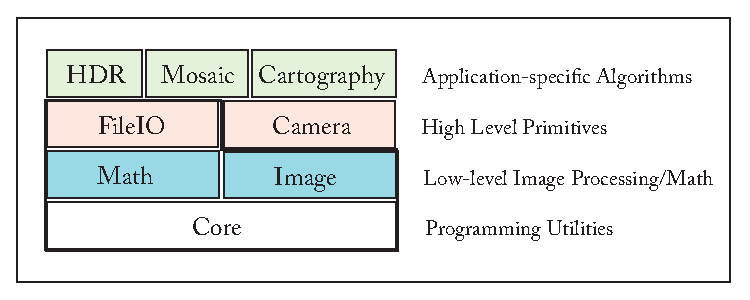
\includegraphics[width=6in]{images/module_dependencies.pdf}
 \end{center}
  \label{fig:module-dependencies}
  \caption{{\em Vision Workbench inter-module dependencies}.  Module in this
    figure depend on those beneath them.  These dependencies split the
    modules into four general classes of increasing complexity and
    sophistication.  The modules surrounded by the bold outline are
    considered the ``foundation'' modules that are part of the most
    basic Vision Workbench distribution.}
\end{figure}

It is worth mentioning that the Vision Workbench has several
inter-module dependencies that you should take into account when
enabling and disabling modules.  These are shown in Figure
\ref{fig:module-dependencies}.

Two handy options, \verb#--enable-optimize# and \verb#--enable-debug#,
determine the compiler options used when building the few library
files.  You can again specify an optional argument of the form
\verb#=no# to disable the corresponding feature, and you can also
specify a particular optimization level in the same manner.  For
example, if you want to make it as easy as possible to debug Vision
Workbench code using a debugger you might use
\verb#--enable-optimize=no --enable-debug# to disable all
optimizations and include debugging symbols.  The corresponding
configuration file variables are \verb#ENABLE_OPTIMIZE# and
\verb#ENABLE_DEUBG#.  Keep in mind that since most Vision Workbench
code is header-only you should remember to configure your own project
similarly or you may not notice any difference.  For normal
non-debugging use, we strongly recommend that you enable moderate
compiler optimization; much of the heavily templatized and generic
Vision Workbench code requires basic optimizations such as function
inlining to achieve a reasonable level of performance.

Finally, to specify that the build system should install the Vision Workbench 
someplace other than \verb#/usr/local#, specify the path using the 
\verb#--prefix=PATH# option.   The corresponding configuration file 
variable is, of course, called \verb#PREFIX#.

\chapter{Working with Images}\label{ch:workingwithimages}

This chapter is designed to be a first introduction to programming 
using the Vision Workbench.  It describes images, pixels, color 
spaces, image file I/O, and basic image manipulation, setting the 
stage for the fundamental image processing operations described in 
Chapter~\ref{ch:imageprocessing}.

\section{The {\tt ImageView} Class}

The \verb#ImageView# class is the centerpiece of the Vision Workbench 
in most applications.  Simply put, it represents an image in memory. 
The class is similar to related classes that appear in other C++ computer 
vision libraries, including VXL, GIL, and VIGRA, so if you are already 
familiar with one of those libraries you should find nothing too 
foreign here.

\subsection{The Basics}
An \verb#ImageView# represents a two-dimensional rectangular array of
data, such as an image of pixels.  It is actually a class {\it template}, 
and when you declare an \verb#ImageView# object you specify the
particular kind of data that it should contain.  For example, you can
make an \verb#ImageView# of RGB (red/green/blue) pixels to represent a
full-color image or an \verb#ImageView# of vectors to represent a vector 
field.  You specify the pixel type as a template parameter to the 
\verb#ImageView# class like this:
\begin{verbatim}
  ImageView<PixelRGB<float32> > my_image;
\end{verbatim}
In this case we've made a full-color RGB image.  Notice that 
\verb#PixelRGB# is itself a template: here we've specified that we
want each channel of each RGB pixel to be stored as a 32-bit 
floating-point number.  All of the core pixel types in the Vision 
Workbench are themselves templates like this.

The \verb#ImageView# class is defined in the C++ header file
\verb#<vw/Image/ImageView.h>#, and the standard pixel types are
defined in the header \verb#<vw/Image/PixelTypes.h>#.  Thus, for the
above line of code to compile you must include those two headers at
the top of your program.  (Alternatively, all of the header files
relating to basic image manipulation are collected together in the
convenience header \verb#<vw/Image.h>#.)  Furthermore, all of the core
classes and functions of the Vision Workbench are defined in the C++
namespace \verb#vw#.  One way to use them is to be fully specific:
\begin{verbatim}
  vw::ImageView<vw::PixelRGB<vw::float32> > my_image;
\end{verbatim}
The other way, which may be simpler for new users, is to bring the 
entire \verb#vw# namespace into the global scope by saying 
\begin{verbatim}
  using namespace vw;
\end{verbatim}
at the top of your program after you've included the necessary
headers.  For brevity, in the examples in this book we will often
assume that you have included the necessary headers and we will omit
explicit references to namespace \verb#vw#.  The exception to this is
the complete programs, such as \verb#vwconvert.cc#
(Listing~\ref{lst:vwconvert.cc}, above), which are intended to be
fully self-contained.

By default the dimenions of an \verb#ImageView# are zero, which may not 
be what you want.  One option is to specify an image's dimensions when 
we construct it:
\begin{verbatim}
  ImageView<PixelRGB<float> > my_image( 320, 240 );
\end{verbatim}
This creates an image with 320 columns and 240 rows.  If we ever want to 
set or change the size of an image later on in the code we can use the 
\verb#set_size()# method:
\begin{verbatim}
  my_image.set_size( 640, 480 );
\end{verbatim}
You can also find out how many columns or rows an image has using the 
\verb#cols()# and \verb#rows()# methods, respectively:
\begin{verbatim}
  int width = my_image.cols();
  int height = my_image.rows();
\end{verbatim}
Note that when you call \verb#set_size()# with new image dimensions
the Vision Workbench allocates a new chunk of memory of the
appropriate size.  This is a destructive operation: any old data is
not copied into the new buffer, and the old buffer will be
automatically deallocated if no other objects are using it.

Once you've made an \verb#ImageView#, the simplest way to access a 
particular pixel is by indexing directly into it:
\begin{verbatim}
  PixelRGB<float> some_pixel = my_image( x, y );
\end{verbatim}
In this example we've assumed that \verb#x# and \verb#y# are integer
variables with the desired pixel's coordinates.  For a less trivial
example, one way to fill our image with the color red would be to loop
over all the rows and columns, setting each pixel at a time:
\begin{verbatim}
  PixelRGB<float> red(1.0, 0.0, 0.0);
  for ( int y=0; y<my_image.rows(); ++y )
    for ( int x=0; x<my_image.cols(); ++x )
      my_image(x,y) = red;
\end{verbatim}
This is not the fastest way to access the pixels of an image, but 
it is arguably the most flexible.  (Later we will learn about much 
simpler ways to fill an image with a single color.)

\subsection{The Standard Pixel Types}

The Vision Workbench provides a number of standard pixel types that
you can use to manipulate the most common sorts of images.  We've
already encountered \verb#PixelRGB#, the standard RGB pixel type.  As
we mentioned earlier, this is a template class whose template
parameter specifies the underlying numeric data type used to store
each channel of the pixel.  This is called the pixel's {\it channel
  type}.  The Vision Workbench defines convenient platform-independent
names for the standard channel types, so that you never have to worry
about whether \verb#int# or \verb#short# is 16 bits wide on your
platform.  These Vision Workbench channel types are listed in
Table~\ref{tbl:channel-types}.  These are the only channel types with
which the Vision Workbench has been tested, so it is best to stick to
these unless you have a compelling reason not to.

\begin{table}[t]\begin{centering}
\begin{tabular}{|c|l|l|} \hline
Type & Description & Notes \\ \hline \hline
\verb#int8# & Signed 8-bit integer & \\ \hline
\verb#uint8# & Unsigned 8-bit integer & Common for low-dynamic-range imaging \\ \hline
\verb#int16# & Signed 16-bit integer & \\ \hline
\verb#uint16# & Unsigned 16-bit integer & \\ \hline
\verb#int32# & Signed 32-bit integer & \\ \hline
\verb#uint32# & Unsigned 32-bit integer & \\ \hline
\verb#int64# & Signed 64-bit integer & \\ \hline
\verb#uint64# & Unsigned 64-bit integer & \\ \hline
\verb#float32# & 32-bit floating point & Common for high-dynamic-range imaging \\ \hline
\verb#float64# & 64-bit floating point & \\ \hline
\end{tabular}
\caption{The standard Vision Workbench channel types.}
\label{tbl:channel-types}
\end{centering}\end{table}

\begin{table}[t]\begin{centering}
\begin{tabular}{|c|l|l|} \hline
Type & Description & Channels \\ \hline \hline
\verb#PixelGray<T># & Grayscale & Grayscale value (\verb#v#) \\ \hline
\verb#PixelGrayA<T># & Grayscale w/ alpha & Grayscale value (\verb#v#), alpha (\verb#a#) \\ \hline
\verb#PixelRGB<T># & RGB & Red (\verb#r#), green (\verb#g#), blue (\verb#b#) \\ \hline
\verb#PixelRGBA<T># & RGB w/ alpha &  Red (\verb#r#), green (\verb#g#), blue (\verb#b#), alpha (\verb#a#) \\ \hline
\verb#PixelHSV<T># & HSV & Hue (\verb#h#), saturation (\verb#s#), value (\verb#v#) \\ \hline
\verb#PixelXYZ<T># & XYZ & CIE 1931 X (\verb#x#), Y (\verb#y#), and Z (\verb#z#) channels \\ \hline
\verb#Vector<T,N># & An \verb#N#-dimensional vector & \verb#N# vector components \\ \hline
\verb#T# & A unitless scalar & N/A \\ \hline
\end{tabular}
\caption{The standard Vision Workbench pixel types.  The channel 
type {\tt T} should generally be one of the types from Table~\ref{tbl:channel-types}.}
\label{tbl:pixel-types}
\end{centering}\end{table}

The standard pixel types are listed in Table~\ref{tbl:pixel-types}.
The first four, used for grayscale and RGB images with and without
alpha channels, are the most common.  (For those of you who are 
unfamiliar with the term, an {\it alpha} channel is used to represent 
the opacity of a pixel.  For the rest of you, note that the Vision 
Workbench generally stores alpha pixels in premultiplied form.)

Each of the channels in a pixel can be accessed by indexing into it
directly, as in \verb#my_pixel(i)# or \verb#my_pixel[i]#.  The order 
of the channels is the same as the order in which they appear in the 
name of the type.  If you know a particular pixel's type you can also 
access it's channels by name, so for example \verb#my_rgb_pixel.r()# 
access an RGB pixel's red channel.  (Note that grayscale values are 
accessed via \verb#v()#, for ``value''.)

When you are writing Vision Workbench programs you may often find 
yourself working with only one pixel type at a time.  In this case 
it can be convenient to place a \verb#typedef# near the top of your 
file defining a convenient shorthand:
\begin{verbatim}
  typedef vw::ImageView<vw::PixelRGB<float32> > Image;
\end{verbatim}
This way you can refer to your RGB image type by the much shorter
identifier \verb#Image#.  In the remainder of this book when we say
\verb#Image# you may assume that you may substitute the
\verb#ImageView# class type that is most appropriate for your
application.

Standard conversions are provided among all the RGB and grayscale pixel 
types, and also between \verb#PixelRGB# and the special color types 
\verb#PixelHSV# and \verb#PixelXYZ#.  The \verb#ImageView# class can 
take advantage of these pixel conversions to perform color space 
conversion on entire images.  For example, images are generally stored 
on disk in an RGB color space but it is sometimes helpful to convert 
them to HSV for processing.  This is easy with the Vision Workbench:
\begin{verbatim}
  ImageView<PixelRGB<float> > rgb_image;
  read_image( rgb_image, filename );
  // Convert the RGB image to HSV:
  ImageView<PixelHSV<float> > hsv_image = rgb_image;
\end{verbatim}
(We'll have more to say about \verb#read_image()# shortly, but it 
does what you'd expect.)  Later you could assign the HSV image back 
to an RGB image prior to saving it to disk.

\subsection{Copying {\tt ImageView}s}

In the Vision Workbench, \verb#ImageView# objects have {\it shallow
copy semantics}.  That is, when you copy an \verb#ImageView# you're
making a new \verb#ImageView# that points to the {\it same} data,
rather than a new copy of the data.  This is a relatively inexpensive
operation, which makes it perfectly reasonable to do things like
construct a \verb#std::vector# of \verb#ImageView#s.  The underlying
image data is reference-counted, and when the last \verb#ImageView#
stops using a block of image data it is deallocated.

Though this behavior can be quite powerful, it may not always be 
what you want.  If you ever need to make a duplicate of an 
\verb#ImageView#, so that you can modify one without affecting the 
other, you should use the \verb#copy()# function found in 
\verb#<vw/Image/Algorithms.h>#.
\begin{verbatim}
  // This makes a shallow copy, pointing to the same:
  Image new_image_1 = my_image;
  // This makes a deep copy, pointing to new, identical data:
  Image new_image_2 = copy( my_image );
\end{verbatim}

\subsection{{\tt ImageView} as a STL-Compatible Container}

An \verb#ImageView# can be thought of as a container of pixels, and in
fact you can use it as a standard C++ container class.  The iterator
type is, as expected, called \verb#ImageView<T>::iterator#, and it
allows you to access each of the pixels of an image one at a time.
The \verb#begin()# and \verb#end()# methods return iterators pointing
to the first and one-past-the-last pixels, respectively.  The first
pixel is located at postion $(0,0)$, and incrementing the iterator
advances to the next column.  After it passes through the last column,
the iterator wraps around to the beginning of the next row.

This C++ Standard Template Library (STL) compliant iterator exists
mainly to allow you to take advantage of the many {\it algorithms}
provided by the STL that operate on containers.  For example, you can
use \verb#sort()# to sort all of the pixel values in an image.
\begin{verbatim}
  std::sort( my_image.begin(), my_image.end() );
\end{verbatim}
That particular example may be more cute than it is useful, but others
occur more frequently.  For instance, you can use \verb#std::count()# 
to count the number of pixels with a particular value, or
\verb#std::replace()# to replace all pixels that have one value with
another.

\subsection{Image Planes}

The \verb#ImageView# class also supports another feature found in many
other image processing libraries: image planes.  Like duct tape,
planes are the wrong solution to almost every problem, and we
discourage their use.  Basically, planes allow you to store some
number of two-dimensional pixel arrays of the same size (``planes'')
together in a single object.  Planes are different from channels in
that the number and meaning the planes is not specified at compile
time.  This means that the Vision Workbench can not take advantage of
that information as readily: for example, it has no way to know
whether a three-plane image is RGB, HSV, or something altogether
different, and it cannot optimize operations by unrolling inner loops
as it is able to with channels.  (It may not be readily apparent, but
the sample program shown in Listing~\ref{lst:vwconvert.cc}
demonstrates one of the very few possibly-legitimate uses of planes;
this will be discussed more in the following section on File I/O.)

To create a multi-plane image, pass the desired number of planes as a 
third argument to the \verb#ImageView# constructor or to the 
\verb#set_size()# method.  You can query the number of planes in an 
image with the \verb#planes()# method.  To access a pixel in particular 
plane of an image, pass the plane as a third argument when indexing 
into the image.
\begin{verbatim}
  Image my_image(320,240,3);      // A 3-plane image
  my_image.set_size(320,240,3);   // Same here
  int planes = my_image.planes(); // Now planes == 3
  Pixel pix = my_image(x,y,p);    // Access a pixel
\end{verbatim}
Once again, if you are thinking about using planes we encourage you to
first consider these alternatives.  If you want a way to store a
collection of related images, consider using a \verb#std::vector# of
\verb#ImageView#s instead.  If you just want to store a bunch of
numbers at each pixel location, consider using \verb#Vector<T,N># as a
pixel type.

\section{Image File I/O}

The most common way to get image data into and out of the Vision Workbench 
is by loading and saving images using file I/O.  There are several mechanisms 
for doing this, varying in complexity, flexibility and (for the time being) 
completeness of implementation.

\subsection{Reading and Writing Image Files}

The simplest method for file I/O is to use the \verb#read_image()# and 
\verb#write_image()# functions, passing them an \verb#ImageView# and 
the filename of the image file on disk that you would like to read from 
or write to.
\begin{verbatim}
  read_image( image, filename );
  write_image( filename, image );
\end{verbatim}
Notice that the order of arguments to these two functions is reversed: 
in both cases the destination is first and the source second.

Both functions determine the image file type by looking at the 
extension of the filename that you provide them.  The exact set of 
file formats that are supported depends on which file format libraries 
the Vision Workbench found on your system when you build it.  For 
example JPEG support depends on \verb#libjpeg#, and so forth.  The 
file formats that the Vision Workbench is designed to support are 
listed in Table~\ref{tbl:file-formats}.  Note that the file extensions 
are case-insensitive.

\begin{table}[t]\begin{centering}
\begin{tabular}{|c|l|l|} \hline
Name & Extension(s) & Description \\ \hline \hline
PNG & \verb#.png# & Standard for lossless compression \\ \hline
JFIF/JPEG & \verb#.jpg#, \verb#.jpeg# & Standard for lossy compression, no alpha \\ \hline
TIFF & \verb#.tif#, \verb#.tiff# & Highly flexible, complicated \\ \hline
OpenEXR & \verb#.exr# & High dynamic range \\ \hline
PDS & \verb#.img# & Planetary Data System images \\ \hline
%PBM & \verb#.pnm#, \verb#.ppm#, \verb#.pgm# & Highly portable, simplistic \\ \hline
%BMP & \verb#.bmp# & The old Windows format \\ \hline
\end{tabular}
\caption{The standard Vision Workbench image file formats.  Which formats 
your installation supports depends on what supporting libraries you have 
installed.  Adding support for additional file formats is discussed in 
Chapter~\ref{ch:advanced-topics}.}
\label{tbl:file-formats}
\end{centering}\end{table}

Image data on disk is generally stored with one of the four standard
pixel types: grayscale or RGB with or without alpha.  The image
reading and writing routines will freely convert between these
formats.  You should generally create an \verb#ImageView# with the
pixel type that you would like to work with and let the file I/O
system take care of the rest.
\begin{verbatim}
  ImageView<PixelGrayA<float> > image;
  read_image( image, "some_file.jpg" );
\end{verbatim}
In this example we loaded in a JPEG image file (which has an RGB pixel
format) and then converted the data grayscale and padded it with a
constant alpha value of $1.0$, corresponding to fully opaque.  
Attempting to save this image back as a JPEG file would reverse the 
conversion.  (Any transparency is composited on to a black background 
whenever the alpha channel is removed.)

\subsection{More Sophisticated File I/O}

We will only provide an overview of the more advanced file I/O 
techniques here.  Many of them are partially (in some cases barely) 
implemented.  If you want to use any of these features you can 
learn more about them in Chapter~\ref{ch:advanced-topics}.

Images on disk are handled via an abstract image resource
class, called \verb#DiskImageResource# and defined in
\verb#<vw/FileIO/DiskImageResource.h>#.  You can create one directly 
using the same file-extension-based file type deduction mechanism 
discussed above.
\begin{verbatim}
  DiskImageResource *dir1 = DiskImageResource::open( filename );
  DiskImageResource *dir2 = DiskImageResource::create( filename, format );
\end{verbatim}
In the first case we are opening an existing file, and in the second 
case we are creating a new file.  Creating a new file resource requires 
providing some hints about the underlying image format, such as its 
dimensions and pixel type, which are supplied by a \verb#GenericImageFormat# 
object.

Once you have a resource you can query it for information about its 
dimensions, pixel format and channel type.  For example, you can choose 
to process different pixel formats differently.
\begin{verbatim}
  switch( dir1->pixel_format() ) {
    case VW_PIXEL_GRAY: /* process grayscale file */ break;
    case VW_PIXEL_RGB:  /* process RGB file */       break;
    /* ... */
  }
\end{verbatim}
You can use the \verb#DiskImageResource#'s \verb#read()# and \verb#write()# 
methods to read the data into or write the data out of an \verb#ImageView#, 
respectively.

If you wish to force a particular file format, you can create a resource 
object of the appropriate type directly.
\begin{verbatim}
  DiskImageResourcePNG *dirp1 = new DiskImageResourcePNG( filename );
  DiskImageResourcePNG *dirp2 = new DiskImageResourcePNG( filename, format );
\end{verbatim}
In thise case we show how to create PNG image resources.  If you do this 
then you can take advantage of any special services provided by the 
particular file format's resource type, such as the ability to read or 
write special file header information.

Finally, you can make a read-only \verb#ImageView#-like object that 
corresponds to an image on disk.  This is called a \verb#DiskImageView# 
and is defined in the header of the same name.  This can be used to 
process images that are too large to be loaded into memory all at once. 

\section{Manipulating Images}

We have seen how images are represented via the \verb#ImageView#
class, how to save and load them to and from disk, and how to
manipulate their pixels individually.  Now it is time to begin 
discussing how to perform slightly higher-level operations on images.

\subsection{Simple Image Manipulation}
\label{sec:simple-image-manipulation}

We begin with the simple image manipulation functions listed in
Table~\ref{tbl:image-manipulation} and defined in the header file
\verb#<vw/Image/Manipulation.h>#.  Many of these should be
self-explanatory.  The results of applying several of these transforms
to an image are shown in
Figures~\ref{fig:simple.rotate180}--\ref{fig:simple.subsample}.  The
90-degree rotation functions are one of the few places where the
Vision Workbench makes any kind of assumption about the interpretation
of the $x,y$ coordinate system.  When it is necessary to make a
distinction we assume that the origin $(0,0)$ is the top-left corner
of the image.  If you have been interpreting the origin as the
top-right or bottom-left you will need to invert your notion of
clockwise vs. counter-clockwise when calling these two functions.

None of these functions, by themselves, modify image data or produce 
new images.  Instead, each function returns a special {\it view} 
on to the same image data.  In most cases you will assign the result 
to another \verb#ImageView#, causing the data to be processed and 
the resulting image to be stored in the new buffer:
\begin{verbatim}
  image2 = flip_vertical( image1 );
\end{verbatim}
It's worth taking a moment to study exactly what goes on behind 
the scenes when you perform an operation like this.  First the 
Vision Workbench resizes the destination image (\verb#image2# 
in the above example) if necessary so that its dimensions are 
the same as those of the source image (a flipped version of 
\verb#image1#).  Second it computes the result of the operation, 
storing the result in the destination image as it goes.  The 
important point is that if the destination image already has the 
same dimensions as the source image then it is {\it not} resized 
or reallocated.  This avoids unnecessary memory allocations in 
common situations, such as when you are processing many 
identically-sized images in a loop.  However, it also means that 
you must be careful when processing an image and assigning it back 
to itself:
\begin{verbatim}
  image = flip_vertical( image );   // Bad idea: self-assignment
\end{verbatim}
In this example, the destination image clearly has the same 
dimensions as the source (since they are the same image) and so 
no new image buffer is allocated.  As a result the 
\verb#flip_vertical# operation will clobber the source image with 
partial results, producing garbage.  One solution to this problem 
is to force the creation of a temporary buffer using the \verb#copy# 
function:
\begin{verbatim}
  image = copy( flip_vertical( image ) );   // Much better
\end{verbatim}

\begin{table}[t]\begin{centering}
\begin{tabular}{|c|l|l|} \hline
Function & Description \\ \hline \hline
\verb#rotate_180(im)# & Rotate the image 180 degrees \\ \hline
\verb#rotate_90_cw(im)# & Rotate the image 90 degrees clockwise \\ \hline
\verb#rotate_90_ccw(im)# & Rotate the image 90 degrees counter-clockwise \\ \hline
\verb#flip_vertical(im)# & Flip the image vertically \\ \hline
\verb#flip_horizontal(im)# & Flip the image horizontally \\ \hline
\verb#transpose(im)# & Transpose the \verb#x# and \verb#y# coordinates of the image \\ \hline
\verb#crop(im,x,y,c,r)# & Crop the image, specifying $(x,y)$ and $(cols,rows)$ \\ \hline
\verb#crop(im,bbox)# & Crop the image, specifying a bounding box \\ \hline
\verb#subsample(im,factor)# & Subsample the image by an integer factor \\ \hline
\verb#subsample(im,xfac,yfac)# & Subsample the image by integer factors in $x$ and $y$ \\ \hline
\verb#select_col(im,col)# & Refers to an individual column of an image \\ \hline
\verb#select_row(im,row)# & Refers to an individual row of an image \\ \hline
\verb#select_plane(im,plane)# & Refers to an individual plane of an image \\ \hline
\verb#select_channel(im,channel)# & Refers to an individual channel of an image \\ \hline
\verb#channels_to_planes(im)# & Interprets a multi-channel image as a multi-plane image \\ \hline
\hline
\verb#pixel_cast<PixelT>(im)# & Casts an image to a new pixel type \\ \hline
\verb#pixel_cast_rescale<PixelT>(im)# & Casts an image to a new pixel type, with rescaling \\ \hline
\verb#channel_cast<ChanT>(im)# & Casts an image to a new channel type \\ \hline
\verb#channel_cast_rescale<ChanT>(im)# & Casts an image to a new channel type, with rescaling \\ \hline
\verb#planes_to_channels<PixelT>(im)# & Interprets a multi-plane image as a multi-channel image \\ \hline
\verb#weighted_rgb_to_gray(im)# & Converts RGB to grayscale with default weights \\ \hline
\verb#weighted_rgb_to_gray(im,r,g,b)# & Converts RGB grayscale with the given weights \\ \hline
\end{tabular}
\caption{The simple image manipulation functions, defined in the header file 
{\tt <vw/Image/Manipulation.h>}.  The functions in the top section return writable views.}
\label{tbl:image-manipulation}
\end{centering}\end{table}

The functions listed in the upper section of Table~\ref{tbl:image-manipulation} 
all provide new ways of accessing the same data without doing any additional 
processing.  As a result, these functions are all able to return {\it writable} 
views of their image argument.  That is, you can use them to modify an image by 
placing them on the left side of an equals sign.  For example, suppose you want 
to add a small inset to a larger image, by copying a small image into the larger 
one at a particular postion.  One easy way is to specify the destination region 
using the \verb#crop()# function:
\begin{verbatim}
  int cols = small_image.cols(), rows = small_image.rows();
  crop( large_image, xpos, ypos, cols, rows ) = small_image;
\end{verbatim}
Here we've cropped a region of the large image and used it for writing
instead of reading.  Note that the assignment proceeds just as before: 
first the destination image dimensions are checked, and then the data 
is copied.  However in this case the Vision Workbench will throw an 
exception if the dimensions differ, since it is not meaningful to 
``resize'' a cropped region in the same sense that you can freely 
resize an \verb#ImageView#.  This approach can also be used, for example, 
to replace one channel of a multi-channel image using
\verb#select_channel()#.

\begin{figure}[p]
\centering
  \subfigure[{\tt mural} (Original)]{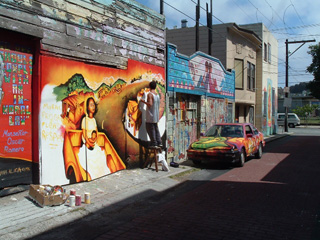
\includegraphics[width=2in]{images/mural.jpg}\label{fig:simple.original}}
  \hfil
  \subfigure[{\tt rotate\char`\_180(mural)}]{\includegraphics[width=2in]{images/mural_rotate_180.jpg}\label{fig:simple.rotate180}}
  \\
  \subfigure[{\tt rotate\char`\_90\char`\_cw(mural)}]{\hbox{\hspace{0.25in}\includegraphics[height=2in]{images/mural_rotate_90_cw.jpg}\hspace{0.25in}\ \label{fig:simple.rotate90cw}}}
  \hfil
  \subfigure[{\tt rotate\char`\_90\char`\_ccw(mural)}]{\hbox{\hspace{0.25in}\includegraphics[height=2in]{images/mural_rotate_90_ccw.jpg}\hspace{0.25in}\ \label{fig:simple.rotate90ccw}}}
  \hfil
  \subfigure[{\tt transpose(mural)}]{\includegraphics[height=2in]{images/mural_transpose.jpg}\label{fig:simple.transpose}}
  \\
  \subfigure[{\tt flip\char`\_vertical(mural)}]{\includegraphics[width=2in]{images/mural_flip_vertical.jpg}\label{fig:simple.flipv}}
  \hfil
  \subfigure[{\tt flip\char`\_horizontal(mural)}]{\includegraphics[width=2in]{images/mural_flip_horizontal.jpg}\label{fig:simple.fliph}}
  \\
  \subfigure[{\tt crop(mural,80,60,160,120)}]{\hbox{\hspace{0.5in}\includegraphics[width=1in]{images/mural_crop.jpg}\hspace{0.5in}\ \label{fig:simple.crop}}}
  \hfil
  \subfigure[{\tt subsample(mural,2)}]{\hbox{\hspace{0.5in}\includegraphics[width=1in]{images/mural_subsample.jpg}\hspace{0.5in}\ \label{fig:simple.subsample}}}
  \\
  \subfigure[{\tt threshold(mural,0.5)}]{\includegraphics[width=2in]{images/mural_threshold.jpg}\label{fig:simple.threshold}}
  \hfil
  \subfigure[{\tt clamp(mural,0.25,0.75)}]{\includegraphics[width=2in]{images/mural_clamp.jpg}\label{fig:simple.clamp}}
\caption{Sample output from the simple image operations discussed in this section.}
\label{fig:simple}
\end{figure}

The functions listed in the lower section of Table~\ref{tbl:image-manipulation}, 
on the other hand, all do a small amount of processing of pixel values.  
The \verb#pixel_cast()# function converts all the pixels in an image to the 
given new pixel type.  The \verb#pixel_cast_rescale()# variants rescale the 
values if the channel type has changed, e.g. mapping the 0--255 range of 
\verb#uint8# on to the $0.0$--$1.0$ nominal range of \verb#float32#.  The 
\verb#channel_*# variants cast the pixels to have the given new channel type, 
leaving the overall pixel format unchanged.  The \verb#pixels_to_channels()# 
function takes a multi-plane image and reinterprets it as a multi-channel 
image with the given pixel type.  Finally, \verb#weighted_rgb_to_gray# converts 
RGB pixels to the corresponding grayscale pixel type using an arbitrary 
weighting of the red, green, and blue channels.  The default weights are 
based on a human perceptual model that weights green most strongly, followed 
by red and then blue.

\subsection{Image Algorithms}

\begin{table}[t]\begin{centering}
\begin{tabular}{|c|l|l|} \hline
Function & Description \\ \hline \hline
\verb#copy(im)# & Produce a deep copy of an image \\ \hline
\verb#fill(im,value)# & Fill an image with a pixel value {\it in-place} \\ \hline
\verb#clamp(im,[low],[high])# & Clamp values to the given range \\ \hline
\verb#normalize(im,[low],[high])# & Normalize values to the given range \\ \hline
\verb#threshold(im,[thresh],[low],[high])# & Threshold an image to two values \\ \hline
\verb#grassfire(im)# & Compute the grassfire image of an image \\ \hline
\verb#bounding_box(im)# & Return the bounding box of an image \\ \hline
\verb#nonzero_data_bounding_box(im)# & Compute the bounding box of nonzero data \\ \hline
\verb#image_blocks(im,width,height)# & Tile an image with bounding boxes \\ \hline
\end{tabular}
\caption{The simple image algorithms defined in the header file {\tt <vw/Image/Algorithms.h>}.}
\label{tbl:image-algorithms}
\end{centering}\end{table}

We will now introduce a number of additional simple image operations
that are defined in the header file \verb#<vw/Image/Algorithms.h>#.
You have already seen one of them, \verb#copy()#, which forces the
creation of a deep copy of an image in a new buffer.  The rest are
listed in Table~\ref{tbl:image-algorithms}.  The result of two of
these functions can be seen in Figures~\ref{fig:simple.threshold}
and~\ref{fig:simple.clamp}.  We hope to implement a number of
additional image algorithms, mirroring the STL container algorithms
but optimized for images, at some point in the future.

The \verb#fill()# function is noteworthy because it is currently the
only core Vision Workbench function that modifies image data {\it
  in-place}.  It is especially useful for filling a single channel of
an image.  For example, you can use it to make an RGBA image fully
opaque.
\begin{verbatim}
  fill( select_channel( rgba_image, 3 ), 1.0 );
\end{verbatim}
(Note that $1.0$ represents fully-opaque if the image has a 
floating-point channel type.)

The \verb#clamp()#, \verb#normalize()#, and \verb#threshold()#
functions return modified versions of their image arguments.
You can assign the result back to the original image, or you can 
save it in a different image instead and keep the original.  
The \verb#clamp()# function clamps the values in the image to 
the given range.  The \verb#normalize# function scales and 
shifts the values of an image so that the values span the 
specified range.  The default range is from zero to the nominal 
maximum value for the channel type, e.g. $1.0$ for floating-point 
images.  This is particularly useful for saving intermediate 
results of your algorithms to disk for debugging.  Finally, the 
\verb#threshold# function returns a two-valued image based on  
whether the pixels in the source image is greater than or less 
than the given threshold value.  The default high and low output 
values are the same as for \verb#norm#, and the default threshold 
is zero.  For example, this line will convert a floating-point 
greyscale image to pure black-and-white:
\begin{verbatim}
  image = threshold( image, 0.5 );
\end{verbatim}

The \verb#grassfire()# algorithm, named for the algorithm that 
it implements, is more specialized.  It takes an image and 
efficiently computes how far each pixel is from from a pixel 
whose value is zero, assuming that pixels outside the image 
boundaries all have zero value.  It measures distance in the 
four-connected Manhattan sense, i.e. as the sum of the 
horizontal and vertical distances.  This algorithm is used in 
a variety of applications, such as avoiding obstacles and 
unknown terrain in path planning.

The final three functions in this section relate to bounding 
boxes, which are the topic of the next section.

\subsection{Bounding Boxes}


\chapter{Image Processing}

Now that we've covered all the basics of how to manipulate images, 
it's time to move on to some more interesting image processing 
tasks.  We begin with an introduction to image filtering, followed 
by a discussion of image math.  We then take a brief detour to 
introduce the Vision Workbench's \verb#Vector# and \verb#Matrix# 
classes before describing image transformation and warping.

By the end of this chapter you will have encoutered all of the core
building blocks that comprise the heart of the Vision Workbench.
There are a number of directions that you can go from here, depending
on what you are hoping to accomplish.  We conclude this chapter with
an overview of the many more specialized features of the Vision
Workbench and a discussion of where to look (in this book and
elsewhere) in order to learn more about them.

\section{Image Filtering}

Image filtering has traditionally been the bread and butter of image
processing software packages.  The Vision Workbench includes a number
of functions to perform the most common filtering operations.  We will
first describe the special-purpose filters, and then we will discuss
the more general convolution-based linear filtering functions.  All of
the filter functions discussed in this section are defined in the
header file \verb#<vw/Filter.h>#.  We will not discuss
frequency-domain filtering in this chapter; that is covered later in
Section~\ref{sec:advanced.frequency}.

\begin{table}[t]\begin{centering}
\begin{tabular}{|c|l|l|} \hline
Function & Description \\ \hline \hline
\verb#gaussian_filter(im,...)# & Apply a Gaussian smoothing filter to an image \\ \hline
\verb#derivative_filter(im,...)# & Apply a discrete differentiation filter to an image \\ \hline
\verb#laplacian_filter(im,...)# & Apply a discrete Laplacian filter to an image \\ \hline
\verb#convolution_filter(im,...)# & Apply a general 2D convolution filter to an image \\ \hline
\verb#separable_convolution_filter(im,...)# & Apply a separable convolution filter to an image \\ \hline
\end{tabular}
\caption{The Vision Workbench image filtering functions, defined in {\tt <vw/Filter.h>}.}
\label{tbl:image-filters}
\end{centering}\end{table}

\subsection{The Special-Purpose Filters}

At the moment only three special-purpose filters are fully supported.
The first is a Gaussian smoothing or blurring filter, which convolves
the image with a discrete Gaussian kernel that has a user-specified
standard deviation (a.k.a. ``sigma'') and user-specified size in each
axis. In order for the filter to accurately approximate a Gaussian,
the size of the kernel should be at least a few times the standard
deviation.  However, unnecessary computation is performed if the size
is much larger than that.  You can omit the size arguments, in which
case the function will pick a kernel size based on your standard
deviation that is reasonable for most applications.  In the most
common case the two standard deviations are equal, in which case you
need only specify a single value for sigma.
\begin{verbatim}
  result = gaussian_filter( image, sigma );
  result = gaussian_filter( image, xsigma, ysigma );
  result = gaussian_filter( image, xsigma, ysigma, xsize, ysize );
\end{verbatim}
In these examples, the \verb#sigma# arguments are generally
floating-point whereas the \verb#size# variables are integers.

The next filter is the derivative filter, which performs a 
discrete spatial differentiation of your image.  Here again, you 
can specify the order of differentiation in the two axes as well 
as the filter kernel size.
\begin{verbatim}
  result = derivative_filter( image, xderiv, yderiv );
  result = derivative_filter( image, xderiv, yderiv, xsize, ysize );
\end{verbatim}
There is a minimum filter size below which it is not possible compute
any given derivative, and these functions will throw an exception if
you try.  For the most part it is a good idea to just let the Vision
Workbench pick the kernel size.

The final special-purpose filter is the Laplacian filter, which 
performs a discrete approximation to the Laplacian operation
$\nabla^2=\frac{d^2}{dx^2}+\frac{d^2}{dy^2}$.
\begin{verbatim}
  result = laplacian_filter( image );
\end{verbatim}
This filter does not take any special parameters.  Note that if you 
are accustomed to using a ``larger'' derivative or Laplacian filter 
to reduce the effect of noise, you are probably better off applying 
a smoothing operation (e.g. via \verb#gauusian_filter()#) first.

\subsection{Edge Extension Modes}

\begin{table}[t]\begin{centering}
\begin{tabular}{|c|l|l|} \hline
Type & Description \\ \hline \hline
\verb#ConstantEdgeExtend# & Assume constant (i.e. nearest-neighbor) edge extension \\ \hline
\verb#ZeroEdgeExtend# & Assume zero-value edge extension \\ \hline
\end{tabular}
\caption{The edge extension modes.}
\label{tbl:edge-extension-modes}
\end{centering}\end{table}

To filter the regions near the edges of an image properly, 
filters like these need to make some sort of assumption 
about the contents of the source image {\it beyond} the 
image boundaries.  This is generally referred to as ``edge 
extension''.  The default assumption made by the filters 
discussed in this section is that in each direction the 
image is extended with a constant value equal to the value 
of the nearest edge pixel.  However, you can specify an 
alternative edge extension mode if you wich, by passing 
an extra argument to the filters.  The C++ type of the 
argument determines the edge extension mode used.  
\begin{verbatim}
  result = gaussian_filter( image, 3.0, ConstantEdgeExtend() );
  result = gaussian_filter( image, 3.0, ZeroEdgeExtend() );
\end{verbatim}
Both of these examples filter the source image using a 
standard deviation of three pixels and an automatically-chosen 
kernel size.  However, the first explicitly requests the 
default edge extension behavior, while the second requests 
that the source image be assumed to be zero outside the 
image boundaries.

Notice the ``extra'' set of parentheses after the names 
of the edge extension modes.  Remember that those names are 
C++ {\it types}, and you can only pass an {\it object} as an 
argument to a function.  Those parentheses invoke the 
edge extension type's constructor, returning a dummy 
object that you pass as the final argument to the filtering 
function.  If you find this confusing, don't worry too much 
about it right now.  Just keep in mind that when you're 
using a type as an argument to a function to change it's 
behavior you need the extra parentheses.  The types that 
are currently supported as edge extension modes are listed 
in Table~\ref{tbl:edge-extension-modes}.

\subsection{General Convolution Filtering}

Most of the filters used in image processing are convolution filters,
which express each output pixel as a fixed weighted sum of neighboring
input pixels.  An image convolution filter is usually described by a
rectangular array of weights called the {\it kernel}.  The easiest way
to think about an image kernel is as the result that you would desire 
from the filter if the input image had the value $1$ at the origin and
zero everywhere else.  (This is also known as the ``impulse response''
of the filter.)  For example, a first-order derivative filter in the
$x$ direction might have the kernel
$[\begin{array}{ccc} 1 & 0 & -1 \end{array}]$.
In this case we also need to know that the middle number of the kernel 
(the zero in this case) is the kernel's origin.

In the Vision Workbench, convolution kernels---which as we've said are 
nothing more than rectangular arrays of numbers---are represented by 
images.  The pixel type for a kernel should generally be a scalar type 
such as \verb#float#.  Once you've put the kernel that you'd like into 
an image it is straightforward to use it to filter another image.
\begin{verbatim}
  ImageView<float> kernel;
  /* set up your kernel here */
  result = convolution_filter( image, kernel );
\end{verbatim}
In this case the Vision Workbench assumes that the center pixel of the
kernel is the kernels's origin.  If this is not what you want then you
can specify the coordinates of the kernel's origin explicitly instead.
\begin{verbatim}
  result = convolution_filter( image, kernel, ox, oy );
\end{verbatim}
In either case you can also optionally specify an edge extension mode, 
just like you could for the special-purpose filters.

Convolution filtering can be computationally expensive if the kernel
is large.  Fortunately, many useful kernels have a special form that
makes it possible to improve the performance considerably.  These are
called {\it separable} kernels, and are themselves the result of
convolving a single-column image with a single-row image.  In other
words, the kernel $K$ must satisfy $K(x,y)=K_x(x)K_y(y)$ for some
functions $K_x$ and $K_y$.  The Gaussian and derivative filters
are both of this form, for example, though the Laplacian filter is
not.

The Vision Workbench provides special support for efficient 
convolution filtering with saseparable kernels.  You must supply the 
{\it separated} kernel, i.e. two one-dimensional kernels.
\begin{verbatim}
  result = separable_convolution_filter( image, xkernel, ykernel );
  result = separable_convolution_filter( image, xkernel, ykernel, ox, oy );
\end{verbatim}
As in the general 2D convolution case, the origin of the kernel is 
assumed to be in the middle if you do not specify otherwise and in 
either case you can add an optional argument specifying the edge 
extension mode.  You can still supply the one-dimensional kernels as 
images, just as you did in the general 2D convolution case, but here 
you can also provide them in another STL-compliant container, such 
as a \verb#std::vector# or (as we shall introduce later this chapter) 
a \verb#vw::Vector#.  If you do chose to represent the kernels as 
images, remember that each should have one of the dimensions set to 1.

\section{Doing Math with Images}

In image processing it is often desirable to perform some mathematical 
operation on every pixel of an image, or to corresponding pixels from 
several images.  For example gamma correction involves applying a 
mathematical function to each pixel, and background subtraction involves
subtracting the corresponding pixels from two images.  In the Vision 
Workbench, these operaations and others like them fall under the rubric 
of ``image math'', and the functions to support them are defined in the 
header \verb#<vw/ImageMath.h>#.

\subsection{Image Operators}

In most cases writing code to perform image math is trivial.  The 
mathematical expressions that you would normally write for individual 
pixels work just as well for whole images of pixels.  For example, 
consider the background subtraction problem mentioned above.
\begin{verbatim}
  result_image = input_image - background_image;
\end{verbatim}
That's all there is to it.  Setting up an IIR lowpass filter to 
estimate the background image is just as easy.
\begin{verbatim}
  background_image = alpha*input_image + (1-alpha)*background_image;
\end{verbatim}
(Here we're assuming that \verb#alpha# is a small positive
floating-point number.)  The important point is that there is no need 
for you to write a loop that performs an operation like this on each 
pixel.  Just write the mathematic expression, replacing pixels with 
images, and you're all set.

\begin{table}[t]\begin{centering}
\begin{tabular}{|c|c|c|c|} \hline
Per-pixel Sum & Per-pixel Difference & Per-pixel Product & Per-pixel Quotient \\ \hline \hline
\verb#image + image#  & \verb#image - image#  & \verb#image * image#  & \verb#image / image#  \\ \hline
\verb#image += image# & \verb#image -= image# & \verb#image *= image# & \verb#image /= image# \\ \hline
\verb#image + value#  & \verb#image - value#  & \verb#image * value#  & \verb#image / value#  \\ \hline
\verb#image += value# & \verb#image -= value# & \verb#image *= value# & \verb#image /= value# \\ \hline
\verb#value + image#  & \verb#value - image#  & \verb#value * image#  & \verb#value / image#  \\ \hline
\end{tabular}
\caption{The Vision Workbench image operators, defined in {\tt <vw/ImageOperators.h>} (which 
is in turn included automatically by {\tt <vw/ImageMath.h>}).}
\label{tbl:image-operators}
\end{centering}\end{table}

This works, of course, because the Vision Workbench has overloaded the
standard C++ mathematical operators to work on images too.  These
operators are listed in Table~\ref{tbl:image-operators}.  Operation
with scalars is treated identically to per-pixel operation with
constant-value images.  In order to simplify division with large
images, the image division operators have been designed so that
division by zero returns zero instead of throwing an exception.

There is one important issue to bear in mind when using image
operators: the underlying per-pixel operations must themselves be
meaningful.  For example, multiplying an image whose pixel type is
\verb#PixelGray# by an image whose pixel type is \verb#PixelRGB# is
not wel-defined, and attempting to do so will result in a compiler
error.  The Vision Workbench will not automatically ``promote'' the
grayscale image to RGB.

This raises the question of what happens when you multiply two images
both of whose pixel type is, for example, \verb#PixelRGB#.  What does
it mean to multiply two RGB colors?  Multiplication is defined defined
for numbers, not colors.  The answer is that in this situation the
Vision Workbench will actually perform the mathematical operation on a
per-{\it channel} basis rather than just a per-pixel basis.

A good rule of thumb when working with image operators is to restrict
yourself to operating on images of the same type, or combinations of
images of one type and images of scalars.  As long as you obey this
rule you should find that the image operators always do what you
expect.

\subsection{Mathematical Functions}

\begin{table}[t]\begin{centering}
\renewcommand\arraystretch{1.2}
\begin{tabular}{|c|c|c|c|} \hline
Function & Description & Function & Description \\ \hline \hline
\verb#sin# & Sine, $\sin x$ & \verb#asin# & Inverse sine, $\sin^{-1} x$ \\ \hline
\verb#cos# & Cosine, $\cos x$ & \verb#acos# & Inverse cosine, $\cos^{-1} x$ \\ \hline
\verb#tan# & Tangent, $\tan x$ & \verb#atan# & Inverse tangent, $\tan^{-1} x$ \\ \hline
\verb#atan2# & \multicolumn{3}{|l|}{Two-argument form of inverse tangent, $\tan^{-1}\!\!\ ^x\!/\!_y$ } \\ \hline
\verb#sinh# & Hyperbolic sine, $\sinh x$ & \verb#cosh# & Hyperbolic cosine, $\cosh x$ \\ \hline
\verb#tanh# & Hyperbolic tangent, $\tanh x$ & \verb#exp# & Exponential, $e^x$ \\ \hline
\verb#log# & Natural logarithm, $\ln x$ & \verb#log10# & Base-10 logarithm, $\log_{10} x$ \\ \hline
\verb#ceil# & Ceiling function, $\lceil x \rceil$ & \verb#floor# & Floor function, $\lfloor x \rfloor$ \\ \hline
\verb#sqrt# & Square root, $\sqrt{x}$ & \verb#pow# & Power function, $x^y$ \\ \hline
\hline
\verb#asinh# & Inverse hyperbolic sine, $\sinh^{-1} x$ & \verb#acosh# & Inverse hyperbolic cosine, $\cosh^{-1} x$ \\ \hline
\verb#atanh# & Inverse hyberbolic tangent, $\tanh^{-1} x$ & \verb#cbrt# & Cube root, $\sqrt[3]{x}$ \\ \hline
\verb#exp2# & Base-2 exponential, $2^x$ & \verb#expm1# & Exponential minus 1, $e^x-1$ \\ \hline
\verb#log2# & Base-2 logarithm, $\log_2 x$ & \verb#log1p# & Lograithm of one-plus, $\ln (1+x)$ \\ \hline
\verb#tgamma# & Gamma function, $\Gamma(x)$ & \verb#lgamma# & Log of Gamma function, $\ln |\Gamma(x)|$ \\ \hline
\verb#hypot# & Hypotenuse, $\sqrt{x^2+y^2}$ & \verb#copysign# & Sign-copying function \\ \hline
\verb#round# & Rounding function & \verb#trunc# & Floating-point truncation \\ \hline
\verb#fdim# & Positive difference, $\max(x-y,0)$ & & \\ \hline
\end{tabular}
\caption{The Vision Workbench image math functions, as defined in {\tt <vw/ImageMath.h>}.
The functions in the bottom section are not available under the Windows operating system.}
\label{tbl:math-functions}
\end{centering}\end{table}

Of course, C++ provides a range of mathematical functions, too, such
as exponentials and logarithms, trigonometric functions, and so forth.
The Vision Workbench extends these functions to operate on images as
well.  The supported functions are listed in
Table~\ref{tbl:math-functions}.  Note that these image functions are
built on top of the standard C++ functions that operate on regular
numbers.  Therefore, the Vision Workbench only supports those
functions that are provided by your platform.  In particular, the
bottom half of Table~\ref{tbl:math-functions} lists functions that are
{\it not} currently available under the Microsoft Windows operating
system.

You can use these functions just like you use the mathematical 
operators: write the same expression that you would write for 
individual pixels, but substitute whole images instead.
\begin{verbatim}
  result_image = pow( input_image, gamma );
\end{verbatim}
This example demonstrates how to use the \verb#pow()# function to 
gamma-correct an image.  (Here we are imagining that the variable 
\verb#gamma# is a floating-point number representing the desired 
gamma correction factor.)  This example also demonstrates the fact 
that either of the arguments of a two-argument mathematical function 
can be a single value instead of an image.  Just as with the operators, 
this is treated the just like a constant-value image.

Note that unlike the normal mathematical functions that C++ inherited
from C, it is not necessary (or correct) to use a different function
name when you are working with \verb#float# image data than you would
use to work with \verb#double# image data.  The function names listed
in Table~\ref{tbl:math-functions} are correct for image math in all
cases.  Those in turn use the proper underlying mathematical functions
as apppropriate---for example, \verb#sin()# invokes \verb#sinf()# on 
each pixel if it is applied to a \verb#float#-based image.

\section{Vectors and Matrices}

Before introducing the next image processing topic, image transformation 
and warping, we must first take a brief detour to introduce the Vision 
Workbench vector and matrix classes.  We will assume in this chapter 
that you have a good familiarity with the underlying mathemtatical 
entities that these classes represent.  Note that our mathematical usage 
of the word ``vector'' here is somewhat different from the C++ standard 
library's use of the word to mean a dynamically-resizable array.

\subsection{Vectors and Vector Operations}

The Vision workbench vector class is called, appropriately enough, 
\verb#Vector#.  Like \verb#ImageView#, \verb#Vector# is a template 
class whose first template parameter is required and specifies the 
underlying numeric type.  However, while the dimensions of an image 
are always specified at run-time via the image's constructor or the 
\verb#set_size()# method, \verb#Vector# comes in two variants.  The 
first form behaves in just the same way, but the second form has a 
fixed size that is specified at compile time.  This eliminates the 
need for frequent dynamic allocation when working with vectors in 
the common case when the vector dimension is known.

Declaring either type of vector is straightforward:
\begin{verbatim}
  Vector<float> vector1(3);
  Vector<float,3> vector2;
\end{verbatim}
Both of those statements declare three-dimensional vectors of 
floating-point numbers.  In the first case the vector is allocated 
dynamically on the heap and the size could have been chosen at 
run-time.  In the second case the vector is allocated statically 
on the stack, but the dimension can {\it not} vary at run time.
The first form is generally useful when, say, reading a large 
vector of data in from a file, while the second form is more 
useful when performing geometric computations.

The second, fixed-dimension form also has special constructors that
you can use to initialize the vector contents:
\begin{verbatim}
  Vector<float,3> vector2(1,2,3);
\end{verbatim}
These constructors are available with up to four arguments.
Alternatively, you can construct both fixed-size and dynamically-sized 
vector with data copied from a block of memory that you point them to:
\begin{verbatim}
  float *some_data;
  Vector<float> vector1(3, some_data);
  Vector<float,3> vector2(some_data);
\end{verbatim}
Remember that this copies the data, so it can be inefficient; see 
the discussion of \verb#VectorProxy# below for an alternative.
Three of the most commonly used vector types have special aliases, 
for convenience:
\begin{verbatim}
  typedef Vector<double,2> Vector2;
  typedef Vector<double,3> Vector3;
  typedef Vector<double,4> Vector4;
\end{verbatim}
These typese are used throughout the remainder of the Vision Workbench 
as the standard geometric vector types.

You can query a vector about its size (i.e. dimension or length) with
the \verb#size()# method, and you can index into a vector to access 
individual elements:
\begin{verbatim}
  for( unsigned i=0; i<vector1.size(); ++i ) vector1(i) = 0;
\end{verbatim}
This example loops over all the elements of a vector, setting them 
to zero.  You can also into a vector with square brackets instead 
of parentheses if you prefer.  For fixed-length vectors there is one 
more way to access up to the first three elements, via methods called 
\verb#x()#, \verb#y()#, and \verb#z()#.
\begin{verbatim}
  vector2.x() = 0;  // Set the first element to zero
\end{verbatim}
These methods are only available if the vector has sufficient 
length.  For example, attempting to use the \verb#z()# method of 
a vector of type \verb#Vector<float,2># will result in a compile-time 
error.  Remember, these methods are only available for fixed-size 
vectors, {\it not} dynamically-sized ones.  Dynamically-sized 
vectors, however, can be resized:
\begin{verbatim}
  vector1.set_size(10);
\end{verbatim}
The \verb#set_size()# function takes an optional second argument that 
specifies whether or not the vector contents should be preserved.  
This argument defaults to \verb#false#, so in the above example 
the old contents (if any) are lost.

\begin{table}[t!]\begin{centering}
\begin{tabular}{|c|l|} \hline
Function & Description \\ \hline \hline
\verb#- vector# & Vector negation \\ \hline
\verb#vector + vector# & Vector sum \\ \hline
\verb#vector - vector# & Vector difference \\ \hline
\verb#vector * scalar# & Scalar product \\ \hline
\verb#scalar * vector# & Scalar product \\ \hline
\verb#vector / scalar# & Scalar quotient \\ \hline
\verb#vector += vector# & Vector sum assignment \\ \hline
\verb#vector -= vector# & Vector difference assignment \\ \hline
\verb#vector *= scalar# & Scalar product assignment \\ \hline
\verb#vector /= scalar# & Scalar quotient assignment \\ \hline
\hline
\verb#elem_sum(vector,vector)# & Elementwise vector sum (same as \verb#+# operator) \\ \hline
\verb#elem_sum(vector,scalar)# & Elementwise sum of a vector and a scalar \\ \hline
\verb#elem_sum(scalar,vector)# & Elementwise sum of a scalar and a vector \\ \hline
\verb#elem_diff(vector,vector)# & Elementwise vector difference (same as \verb#-# operator) \\ \hline
\verb#elem_diff(vector,scalar)# & Elementwise difference of a vector and a scalar \\ \hline
\verb#elem_diff(scalar,vector)# & Elementwise difference of a scalar and a vector \\ \hline
\verb#elem_prod(vector,vector)# & Elementwise product of two vectors \\ \hline
\verb#elem_prod(vector,scalar)# & Elementwise vector product (same as \verb#*# operator) \\ \hline
\verb#elem_prod(scalar,vector)# & Elementwise vector product (same as \verb#*# operator) \\ \hline
\verb#elem_quot(vector,vector)# & Elementwise quotient of two vectors \\ \hline
\verb#elem_quot(vector,scalar)# & Elementwise quotient (same as \verb#/# operator) \\ \hline
\verb#elem_quot(scalar,vector)# & Elementwise quotient of a scalar and a vector \\ \hline
\hline
\verb#norm_1(vector)# & 1-norm of a vector, i.e. $\sum |v_i|$ \\ \hline
\verb#norm_2(vector)# & Euclidean 2-norm of a vector, i.e. $\sqrt{\sum v_i^2}$ \\ \hline
\verb#norm_2_sqr(vector)# & Squared 2-norm of a vector, i.e. $\sum v_i^2$ \\ \hline
\verb#norm_inf(vector)# & Infinity-norm of a vector, i.e. $\max |v_i|$ \\ \hline
\verb#sum(vector)# & Sum of elements, i.e. $\sum v_i$ \\ \hline
\verb#prod(vector)# & Product of elements, i.e. $\prod v_i$ \\ \hline
\verb#normalize(vector)# & The normalized form of a vector, i.e. $v/|v|$ \\ \hline
\verb#dot_prod(vector,vector)# & Vector dot product, i.e. $u\cdot v$ \\ \hline
\verb#cross_prod(vector,vector)# & Vector dot product, i.e. $u\times v$ \\ \hline
\end{tabular}
\caption{The vector math functions defined in {\tt <vw/Vector.h>}.}
\label{tbl:vector-functions}
\end{centering}\end{table}

The \verb#Vector# classes support the standard mathematical operations
of vector addition and subtraction and scalar multiplication and
division via the usual C++ operators.  They also support the a range
of elementwise mathematical operations, such as adding a scalar to
each element or multiplying the corresponding elements of two vectors,
via functions of the form \verb#elem_*#.  There are a number of vector
norms and related functions, as well as a vector dot product and cross
product.  (The cross product is, of course, only valid for
three-dimensional vectors.)  The complete list of vector math
functions defined in \verb#<vw/Vector.h># is given in
Table~\ref{tbl:vector-functions}.

A \verb#Vector# object is also a container in the C++ Standard Template 
Library sense of the word.  There is a \verb#Vector<...>::iterator# type 
that serves as the vector's iterator, and there are \verb#begin()# and 
\verb#end()# methods that return iterators to the first and one-past-the-last 
elements, as usual.  This can be an extremely convienient way to load 
data into and out of \verb#Vector#s.

You can extract a portion of a vector using the \verb#subvector()#
function, which takes three arguments: the original vector, the
position of the first element to extract, and the number of elements
in the resulting vector:
\begin{verbatim}
  Vector<float,3> vector2 = subvector(vector1,5,3);
\end{verbatim}
This example copies the fifth, sixth, and seventh elements of
\verb#vector1# into a new three-element vector.

The streaming operator \verb#<<# is also defined for writing vectors
to C++ output streams, which you can use to dump vector contents for
debugging:
\begin{verbatim}
  Vector<float,3> vector2(1,2,3);
  std::cout << vector2 << std::endl;
  // The output is: [3](1,2,3)
\end{verbatim}
Note that the size of the vector is printed first, followed by the 
vector's contents.

Sometimes it can be useful to work with data that is already stored in 
memory as though it were stored in a \verb#Vector# object.  As long as 
the data is stored in the usual packed format this is easy to do using 
the special \verb#VectorProxy# type, which also comes in fixed-size 
and dynamically-sized variants:
\begin{verbatim}
  float some_data[10] = {0,1,2,3,4,5,6,7,8,9};
  VectorProxy<float> proxy1(10, some_data);
  VectorProxy<float,10> proxy2(some_data);
\end{verbatim}
The constructor arguments are the same as are used in \verb#Vector# to
initialize a vector with data from a block of memory, except the data
is not copied.  You can now treat these proxy objects just like the
were regular \verb#Vector#s, except the contents will be stored in the
region of memory that you pointed them to.  In some situations this
can be considerably more efficient than copying the data
unnecessarily. (It is of course not possible to resize a
\verb#VectorProxy#, since the proxy does not have any control over the
memory that it is using.)

\subsection{Matrices and Matrix Operations}

The Vision workbench \verb#Matrix# class is the matrix 
counterpart to the \verb#Vector# class, and behaves quite 
similarly.  Once again, there are fixed-dimension and 
dynamically-sized versions:
\begin{verbatim}
  Matrix<float> matrix1(3,3);
  Matrix<float,3,3> matrix2;
\end{verbatim}
Note that the arguments to matrix-related functions such 
as these constructors are given in $i,j$ order, i.e. row 
followed by column.  This is {\it different} from images, 
where areguments are given in $x,y$ order, i.e. column 
followed by row.  You may find this confusing at first if 
you are moving to the Vision Workbench from an environment 
like Matlab where there is no distinction between images 
and matrices.  However, it is in keeping with the standard 
index ordering seen in the bulk of the image processsing 
and mathematics literatures, respectively.

You can initialize the matrix with data already stored 
in memory, as long as the data is stored in a packed 
row-major format:
\begin{verbatim}
  float some_data[4] = {1,2,3,4};
  Matrix<float> matrix1(2,2,some_data);
  Matrix<float,2,2> matrix2(some_data);
\end{verbatim}
As in the case of \verb#Vector#, the initialization data 
is {\it copied} into the matrix in this case, but there is 
also a proxy form that allows you treat in-memory data 
like an ordinary matrix:
\begin{verbatim}
  float some_data[4] = {1,2,3,4};
  MatrixProxy<float> matrix1(2,2,some_data);
  MatrixProxy<float,2,2> matrix2(some_data);
\end{verbatim}
The three most common matrix types have been given 
convenient aliases:
\begin{verbatim}
  typedef Matrix<double,2,2> Matrix2x2;
  typedef Matrix<double,3,3> Matrix3x3;
  typedef Matrix<double,4,4> Matrix4x4;
\end{verbatim}
These types are again the standard types used throughout the Vision 
Workbench in geometric applications.

You can query a matrix's dimensions using the \verb#rows()# and 
\verb#cols()# methods, and can index into the matrix to access 
individual elements.  There are two ways to do that:
\begin{verbatim}
  matrix(row,col) = 1;    // "New"-style indexing
  matrix[row][col] = 1;   // "Old"-style indexing
\end{verbatim}
A dynamically-sized matrix can be resized using the 
\verb#set_size()# method:
\begin{verbatim}
  matrix.set_size(rows,cols);
\end{verbatim}
As in the case of resizing vectors, the default behavior is that any
old data is not saved.  The \verb#set_size()# method takes an optional
third boolean parameter that can be set to \verb#true# to request that
it preserve the overlapping entries.

\begin{table}[t!]\begin{centering}
\begin{tabular}{|c|l|} \hline
Function & Description \\ \hline \hline
\verb#- matrix# & Matrix negation \\ \hline
\verb#matrix + matrix# & Matrix sum \\ \hline
\verb#matrix - matrix# & Matrix difference \\ \hline
\verb#matrix * scalar# & Scalar product \\ \hline
\verb#scalar * matrix# & Scalar product \\ \hline
\verb#matrix / scalar# & Scalar quotient \\ \hline
\verb#matrix += matrix# & Matrix sum assignment \\ \hline
\verb#matrix -= matrix# & Matrix difference assignment \\ \hline
\verb#matrix *= scalar# & Scalar product assignment \\ \hline
\verb#matrix /= scalar# & Scalar quotient assignment \\ \hline
\hline
\verb#matrix * matrix# & Matrix product \\ \hline
\verb#matrix * vector# & Matrix-vector product \\ \hline
\verb#vector * matrix# & Vector-matrix product \\ \hline
\hline
\verb#elem_sum(matrix,matrix)# & Elementwise matrix sum (same as \verb#+# operator) \\ \hline
\verb#elem_sum(matrix,scalar)# & Elementwise sum of a matrix and a scalar \\ \hline
\verb#elem_sum(scalar,matrix)# & Elementwise sum of a scalar and a matrix \\ \hline
\verb#elem_diff(matrix,matrix)# & Elementwise matrix difference (same as \verb#-# operator) \\ \hline
\verb#elem_diff(matrix,scalar)# & Elementwise difference of a matrix and a scalar \\ \hline
\verb#elem_diff(scalar,matrix)# & Elementwise difference of a scalar and a matrix \\ \hline
\verb#elem_prod(matrix,matrix)# & Elementwise product of two matrixs \\ \hline
\verb#elem_prod(matrix,scalar)# & Elementwise matrix product (same as \verb#*# operator) \\ \hline
\verb#elem_prod(scalar,matrix)# & Elementwise matrix product (same as \verb#*# operator) \\ \hline
\verb#elem_quot(matrix,matrix)# & Elementwise quotient of two matrixs \\ \hline
\verb#elem_quot(matrix,scalar)# & Elementwise quotient (same as \verb#/# operator) \\ \hline
\verb#elem_quot(scalar,matrix)# & Elementwise quotient of a scalar and a matrix \\ \hline
\hline
\verb#norm_1(matrix)# & Matrix 1-norm \\ \hline
\verb#norm_2(matrix)# & Matrix 2-norm \\ \hline
\verb#norm_frobenius(matrix)# & Matrix Frobenius norm \\ \hline
\verb#sum(matrix)# & Sum of elements, i.e. $\sum v_i$ \\ \hline
\verb#prod(matrix)# & Product of elements, i.e. $\prod v_i$ \\ \hline
\verb#trace(matrix)# & Matrix trace, i.e. $\sum M_{ii}$ \\ \hline
\verb#transpose(matrix)# & Matrix transpose, i.e. $M^T$ \\ \hline
\verb#inverse(matrix)# & Matrix inverse, i.e. $M^{-1}$ \\ \hline
\end{tabular}
\caption{The matrix math functions defined in {\tt <vw/Matrix.h>}.}
\label{tbl:matrix-functions}
\end{centering}\end{table}

Once you've made one or more matrices you can use a wide range of 
mathematical operator and functions to manipulate them.  The 
standard C++ operators, elementwise math functions, and a number 
of other functions similar to those for vectors are supported.  A 
list of the matrix math functions is given in Table~\ref{tbl:matrix-functions}.
Notice that some of these functions also operate with vectors: 
all vector functions that involve matrices are defined in 
\verb#<vw/Matrix.h># instead of \verb#<vw/Vector.h>#.

There is a special method, \verb#set_identity()#, that can be used 
to set a square matrix to the identity matrix of that size.
\begin{verbatim}
  Matrix<float> id(3,3);
  id.set_identity();
\end{verbatim}
If you want to treat a single row or column of a matrix as though 
it were a vector, you can do so using the \verb#select_row()# and 
\verb#select_col()# function:
\begin{verbatim}
  Vector<float> first_row = select_row(matrix,1);
  select_column(matrix,2) = Vector3(1,2,3);
\end{verbatim}
The second of these examples illustrates that you can use the 
\verb#select_*# functions to write into matrix rows and 
columns as well as read them out.  Finally, you can treat 
a block of a matrix as a smaller matrix in its own right 
using the \verb#submatrix()# function:
\begin{verbatim}
  Matrix<float> block = submatrix(matrix,row,col,rows,cols);
\end{verbatim}
You can also use this function to write into a region of a 
matrix, much as in the previous example using \verb#select_col()#.

Like \verb#Vector#, \verb#Matrix# is a C++ STL-compatible 
container class.  The \verb#Matrix<...>::iterator# iterates 
over the elements of a matrix in the same order that the 
\verb#ImageView#'s iterator does: across each row, moving 
down the matrix from each row to the next.  This is again a 
good method for loading or extracting matrix data from other 
containers.  To extract the matrix data to a stream for 
debugging output you can use the \verb#<<# stream output 
operator:
\begin{verbatim}
  double data[4] = {1,2,3,4};
  Matrix2x2 matrix(data);
  std::cout << matrix << std::endl;
  // The output is: [2,2]((1,2)(3,4))
\end{verbatim}
Again, the output includes the matrix dimensions (rows 
followed by cols), followed by the matrix data.

\section{Transforming or Warping Images}

\section{Where to Go from Here}

\chapter{The Core Vision Workbench Type System}

The Vision Workbench is an example of what is often called a
``multiparadigm'' C++ library.  That is, different components of the
library adopt different C++ programming models, such as the generic
programming model or the object-oriented programming model, often in
combination.  At the core, however, is a set of data types and related
tools that fall largely within the template-based generic programming
paradigm.  The purpsoe of this chapter is to describe this core type
system in some detail.  If your intention is simply to {\it use} the
Vision Workbench for image processing tasks you can probably afford
to skim or even skip this material.  The primary intended audience is
programmers who wish to extend the Vision Workbench's core
capabilities in one way or another.

Data types in the Vision Workbench can be broadly divided into three
categories: the fundamental data types, including the simple numeric
types; the compound types, such as RGB pixel types and vectors; and
the container types, such as images.  We shall discuss each of these
in turn.  (Other C++ types, such as functors, do make an appearance in
the Vision Workbench, but these are not {\it data} types {\it per se}.)

\section{The Scalar Types}

\begin{table}[t]\begin{centering}
\begin{tabular}{|c|l|l|} \hline
Type & Description & Notes \\ \hline \hline
\verb#int8# & Signed 8-bit integer & \\ \hline
\verb#uint8# & Unsigned 8-bit integer & Most common for low-dynamic-range imaging \\ \hline
\verb#int16# & Signed 16-bit integer & \\ \hline
\verb#uint16# & Unsigned 16-bit integer & \\ \hline
\verb#int32# & Signed 32-bit integer & \\ \hline
\verb#uint32# & Unsigned 32-bit integer & \\ \hline
\verb#int64# & Signed 64-bit integer & \\ \hline
\verb#uint64# & Unsigned 64-bit integer & \\ \hline
\verb#float32# & 32-bit floating point & Most common for high-dynamic-range imaging \\ \hline
\verb#float64# & 64-bit floating point & \\ \hline
\end{tabular}
\caption{The core Vision Workbench scalar {\tt typedef}s, defined in {\tt <vw/FundamentalTypes.h>}.}
\label{tbl:scalar-types}
\end{centering}\end{table}

The most fundamental data types of all are the built-in C++ integral
and floating-point numeric types.  In scientific programming contexts 
like image processing and machine vision it is generally imporant to 
be able to specify the exact nature of the numeric data types that you 
are working with.  Unfortunately the C++ language makes few promises 
about the sizes of data types such as \verb#int# or even \verb#char#.  
To work around this limitation, the Vision Workbench provides a number 
of portable \verb#typedef#s that you are encouraged to use instead.  
These are listed in Table~\ref{tbl:scalar-types}.  (In fact most of 
these data types are simple wrappers around similar types provided 
by the Boost \verb#cstdint# library.)

The Vision Workbench uses standard C++ complex numbers, as defined 
in the standard header file \verb#<complex>#.  The \verb#std::complex<># 
class takes a single template parameter, the underlying numeric type 
to be used for the real and imaginary components, which should usually 
be one of the scalar types listed in Table~\ref{tbl:scalar-types}. 
In particular, it is almost always best to use one of the floating-point 
types for complex numbers.  For example, \verb#std::complex<float64># 
is a good choice for use in frequency-domain image processing 
(discussed in Section~\ref{sec:advanced.frequency}).

There is a special type trait template, \verb#IsScalar<>#, that you 
can use in template code to determine whether or not a type is a 
simple numeric type like we have described in this section.  It 
inherits from either \verb#boost::true_type# or \verb#boost::false_type# 
accordingly.  Its primary use is to prevent template functions such 
as scalar multiplication from being too general:
\begin{verbatim}
  template <class ScalarT>
  typename boost::enable_if< IsScalar<ScalarT>, MyClass >::type
  operator*( MyClass const& m, ScalarT s ) {
    /* compute result */
  }
\end{verbatim}
In this example we use the Boost \verb#enable_if# library to restrict 
the definition of the \verb#*# operator to cases where the second 
argument really is a scalar.  Without this restriction this would 
have been an overly-general function definition and would likely 
have caused problems if we had attempted to defined any other  
product for the \verb#MyClass# class later on.  If you decide to 
extend the Vision Workbench to support additional scalar types, 
such as bigints, you should specialize \verb#IsScalar<># accordingly 
to ensure proper behavior.

\section{Type Deduction}

\begin{table}[t]\begin{centering}
\begin{tabular}{|c|l|} \hline
Class & Description \\ \hline \hline
\verb#SumType<T1,T2># & Result type of a sum operation \\ \hline
\verb#DifferenceType<T1,T2># & Result type of a difference operation \\ \hline
\verb#ProductType<T1,T2># & Result type of a product operation \\ \hline
\verb#QuotientType<T1,T2># & Result type of a quotient operation \\ \hline
\end{tabular}
\caption{The Vision Workbench type deduction classes, defined in {\tt <vw/TypeDeduction.h>}.}
\label{tbl:type-deduction}
\end{centering}\end{table}

The C++ language has many intricate rules for type promotion and
deduction in complex mathematical expressions.  Unfortunately it
provides no built-in mechanism to extend this automatic type deduction
system or query its behavior.  Consider adding two images with 
compatible but different pixel types: what should the resulting 
pixel type be?  The Vision Workbench provides a standard set of type 
deduction traits classes, defined in \verb#<vw/TypeDeduction.h># and 
listed in Table~\ref{tbl:type-deduction}, that allow you to both query 
and specialize the type deduction behavior of Vision Workbench types.  
Like all Vision Workbench type computation classes, they ``return'' 
their result types in a member type named \verb#type#.

As a trivial example, imagine writing a template function that simply 
computes the sum of its two arguments.  What should its return type 
be?  We can use \verb#SumType<># to compute it:
\begin{verbatim}
  template <class T1, class T2>
  inline typename SumType<T1,T2>::type sum( T1 a, T2 b ) {
    return a + b;
  }
\end{verbatim}
Remember that the C++ language does not allow this to be fully
automatic.  If you define a new type with an unusual addition
operator, you will need to manually specialize \verb#SumType<># at the
same time.  However, the most common default behaviors are provided.
For example, any built-in type is assumed to be promoted to any
user-defined type, and any user-defined type operating with itself is
assumed to return itself.  These type deduction classes do also
replicate the standard C++ promotion behavior when used with the
built-in numeric types.

\section{The Pixel Types}

It is possible to use any of the fundamental scalar types described in
the previous section as an \verb#ImageView#'s pixel type.  However in
most circumstances a {\it compound} pixel type, consisting of one or
more channels with associated semantics, is more appropriate.  The 
Vision Workbench provides several compound pixel types corresponding 
to the most common color spaces used in image processing.  These are 
listed in Table~\ref{tbl:color-pixel-types}.  Each is a template 
class taking one template parameter, the scalar type used to store 
the channels.  For example, the native pixel type of a standard JPEG 
image is represented by \verb#PixelRGB<uint8>#.

\begin{table}[t]\begin{centering}
\begin{tabular}{|c|l|l|} \hline
Type & Description & Channels \\ \hline \hline
\verb#PixelGray<T># & Grayscale & Grayscale value (\verb#v#) \\ \hline
\verb#PixelGrayA<T># & Grayscale w/ alpha & Grayscale value (\verb#v#), alpha (\verb#a#) \\ \hline
\verb#PixelRGB<T># & RGB & Red (\verb#r#), green (\verb#g#), blue (\verb#b#) \\ \hline
\verb#PixelRGBA<T># & RGB w/ alpha &  Red (\verb#r#), green (\verb#g#), blue (\verb#b#), alpha (\verb#a#) \\ \hline
\verb#PixelHSV<T># & HSV & Hue (\verb#h#), saturation (\verb#s#), value (\verb#v#) \\ \hline
\end{tabular}
\caption{The Vision Workbench color-space pixel types, defined in {\tt <vw/PixelTypes.h>}.}
\label{tbl:color-pixel-types}
\end{centering}\end{table}

\begin{table}[t]\begin{centering}
\begin{tabular}{|c|l|l|} \hline
Syntax & Description \\ \hline \hline
\verb#PixelChannelType<PixT>::type# & The pixel type's underlying channel type \\ \hline
\verb#PixelNumChannels<PixT>::value# & The number of channels in the pixel type \\ \hline
\verb#PixelChannelCast<PixT,ChT>::type# & The same pixel type with a new channel type \\ \hline
\hline
\verb#PixelIsCompound<PixT># & Is the pixel type a compound type? \\ \hline
\verb#PixelMakeReal<Pixt>::type# & Converts to the corresponding real channel type \\ \hline
\verb#PixelMakeComplex<Pixt>::type# & Converts to the corresponding complex channel type \\ \hline
%\verb#apply_per_pixel_channel(func,pixel)# & The result of applying \verb#func(ch)# to each channel \\ \hline
%\verb#apply_per_pixel_channel(func,pixel1,pixel2)# & The result of applying \verb#func(ch1,ch2)# to each channel \\ \hline
\end{tabular}
\caption{The pixel traits and pixel type computation classes.}
\label{tbl:pixel-traits}
\end{centering}\end{table}

Several type trait classes are provided for use in writing generic 
pixel manipulation code and are listed in Table~\ref{tbl:pixel-traits}.
The first section of the table lists the classes that you must specialize 
when you write a new compound pixel type.  The second section of 
Table~\ref{tbl:pixel-traits} lists convenience types that are defined 
in terms of the other, specialized types. For example, here is how 
the types are specialized for the RGB pixel type:
\begin{verbatim}
  template <class ChannelT>
  struct PixelChannelType<PixelRGB<ChannelT> > {
    typedef ChannelT type;
  };

  template <class ChannelT>
  struct PixelNumChannels<PixelRGB<ChannelT> > {
    static const unsigned value = 3;
  };

  template <class OldChT, class NewChT>
  struct PixelChannelCast<PixelRGB<OldChT>, NewChT> {
    typedef PixelRGB<NewChT> type;
  };
\end{verbatim}
When you define a new pixel type, you will usually want to define a 
provide a similar set of template specializations.  To simplify 
the process, a macro is provided that you can use to automatically 
specialize the templates in the usual manner:
\begin{verbatim}
  VW_DECLARE_PIXEL_TYPE( PixelRGB, 3 );
\end{verbatim}
This macro expands to the same set of template specializations shown
above, describing a pixel type named \verb#PixelRGB# with three
channels.

Note that it is {\it not} necessary to decare a type using this macro,
or even to provide specializations for the traits templates described
above, just to use that type as the pixel type for an image.  These
specializations are only necessary if you want to declare a type with
multi-channel semantics.  For any other type, the default Vision
Workbench behavior is to treat the type as a single-channel pixel type
whose channel type is equal to the type itself.

Several convenience functions are also provided to simplify working
with pixels in generic template functions.  The first is the
\verb#pixel_channel_cast<>()# function, which casts a pixel to a pixel
of the corresponding pixel type but with the specified channel type.
The syntax mirrors the built-in C++ casting functions, except the
template parameter is the new channel type instead of the new type as
a whole.  In the following example we explicitly down-cast the channel
type of a pixel from \verb#float64# to \verb#float32# in order to pass
it to a function that happens to take a \verb#PixelRGB<float32>#
argument:
\begin{verbatim}
  PixelRGB<float64> pixel;
  some_function( pixel_channel_cast<float32>( pixel ) );
\end{verbatim}
Note that this is not needed in the more common case that the 
function that you wish to call is itself generic and can accept 
any channel type.

Sometimes it is desirable to perform apply a function to each channel
of a pixel, or to corresponding channels from two pixels.  Rescaling a
pixel or adding two pixels on a per-channel basis can be cast into
this form, for example.  You can use the generic function
\verb#apply_per_pixel_channel()# to do this.  Here is a trivial 
example that demonstrates rescaling:
\begin{verbatim}
  float32 triple(float32 v) { return 3*v; }
  // Later, in some other function...
  PixelRGB<float> pixel(.1,.2,.3);
  PixelRGB<float> result = apply_per_pixel_channel(&triple,pixel);
\end{verbatim}
In this case it would have been simpler to multiply the pixel 
by $3$ directly, but the point is that we could have performed 
any arbitrarily complex operation on each channel instead.
The binary form simply takes an extra pixel argument:
\begin{verbatim}
  float32 sum(float32 a, float32 b) { return a+b; }
  // Later...
  PixelRGB<float> pixel1(.1,.2,.3), pixel2(.2,.1,.4);
  PixelRGB<float> result = apply_per_pixel_channel(&sum,pixel1,pixel2);
\end{verbatim}

\subsection{Mathematical Operators}
Virtually all image processing operations depend on pixel 
arithmetic in one way or another.

\chapter{The Camera Module}

Cameras are the interface between images and the real world, and as
such, their importance in computer vision cannot be understated.  In
fact, some would say that computer vision algorithms are distinguished
by the fact that they endeavor to associate the processed pixel data
with objects in the real world for the purposed of measurement,
tracking, or display.  This is achieved by modeling the geometric and
physical properties of the device that was used to capture the
original image.  This is the purpose of the camera module.

The camera module includes built-in models for generic pinhole and
line-scan imagers and a set of generic functions for linearizing
(removing lens distortion) and epipolar rectifying (e.g. for stereo)
when these operations are relevant.  These classes and functions can
be imported into your code by including {\tt <vw/Camera.h>}.

Because you will likely encounter new camera geometries not supported
by the built-in classes, the camera module is designed to be
extensible.  You can provide your own camera model by inheriting
from and adopting the interface of the {\tt CameraModel} abstract base
class, which is defined in the header file {\tt <vw/Camera/CameraModel.h>}.

Finally, the camera module provides a basic set of tools for working
with images from real-world camera systems: bayer pattern filtering
and EXIF parsing.  We will cover all of these features in more detail,
but we begin this chapter by establishing some terminology while
exploring the most common camera geometry in use today: the pinhole
camera model.

\section{The Pinhole Camera Model}
The pinhole camera model describes the geometry found in nearly all
commercial digital camera systems today.  It is characterized by a
lens assembly that focuses light onto a two dimensional array of
pixels (usually a sensor with light sensitive circuits such as a CCD
or CMOS device).  We will use the pinhole model to establish some
terminology that will be used throughout the rest of this chapter.  Be
warned that the model we are about to develop is simplistic; many of
the non-ideal characteristics of a real-world optical system
(e.g. lens distortion) are not modeled in this simple example.  Refer
to the CAHVOR model in Section \ref{sec:built-in-cameras} if you
require a pinhole camera model that more accurately models lens
distortion.

\subsection{Perspective Projection}

Figure \ref{fig:pinhole-camera-diagram} shows the geometry of a basic
pinhole camera.  The light gray area represents the 2D array of
pixels, and it is referred to as the {\em image plane}.  The origin of
the 3D coordinate system is the point $C$, which is the center of
projection or {\em camera center} of the imager.  When a 3D point $O$
is imaged by the camera, it appears at the pixel located where segment
$\overline{OC}$ intersects the image plane at point $(u,v)$.  A line
segment $\overline{OC}$ that is perpendicular to the image plane
intersects this plane at the {\em principal point}, $(p_u, p_v)$.

\begin{figure}[tbp]
\begin{center}
  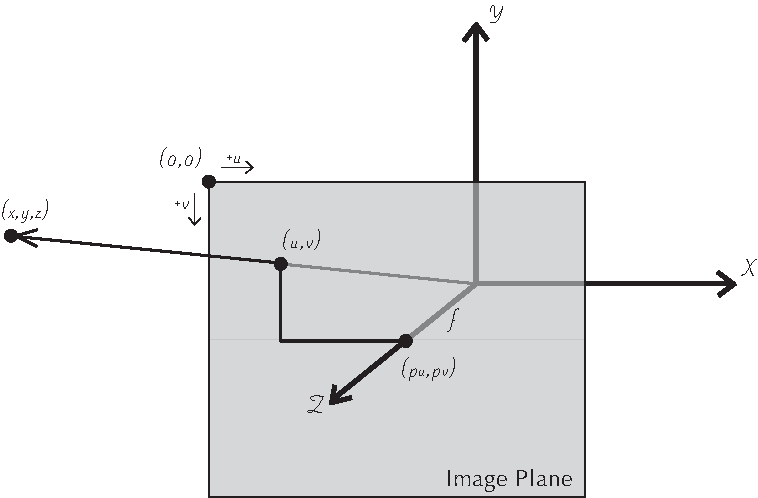
\includegraphics[width=6in]{images/camera_module_pinhole.pdf}
 \end{center}
  \caption{The basic pinhole camera model.}
  \label{fig:pinhole-camera-diagram}
\end{figure}

All of the points imaged by the camera appear on a line that passes
through $C$.  If the coordinates of ${\bf O}$ are $(x,y,z)$, then the
position of the point on the imager can be determined by projecting it
onto the plane $ z = +f$:
\begin{eqnarray}
\label{eqn:forward-projection-1}
u &=& \frac{f}{\sigma} \left(\frac{x}{z}\right) - p_u \\
\label{eqn:forward-projection-2}
v &=& \frac{f}{\sigma} \left(\frac{-y}{z}\right) - p_v
\end{eqnarray}

Here, $f$ is the focal length of the imager in meters, $\sigma$ is the
size of a pixel in {\em m/pixel}, and $(p_u, p_v)$ are the offset in
pixels of the principal point (this offset moves the origin of the
image from the principal point to the upper left hand corner, which is
the ``origin'' usually adopted when indexing images).  

Equations \ref{eqn:forward-projection-1} and
\ref{eqn:forward-projection-2} constitute the {\em forward projection}
portion of the camera model; this is analogous to the process of
``capturing'' an image with a real camera.  Our model should tell us
exactly what what pixel location to look at if you wanted to see the
point $O$ in the image.

Notice how some information is lost during forward projection.  Any
point along $\overline{OC}$ will be imaged to the same point $(u,v)$
on the image plane, so if we were to start with a point $P=(u,v)$ on
the image plane, and we wanted to find the original 3D point $O$, the
best we could do would be to say that it appears somewhere along the
ray $\overrightarrow{CP}$. The
origin and direction of the ray can be computed as follows:

\begin{eqnarray}
\label{eqn:reverse-projection-1}
\overrightarrow{CP}_{origin} & = & C \\
\label{eqn:reverse-projection-2}
\overrightarrow{CP}_{direction} & = & \frac{(u + p_u, -(v + p_v), f)} {||(u + p_u, -(v + p_v), f)||_2}
\end{eqnarray}

This operation, which we call {\em back projection}, can still
provide useful information that can be used in a full 3D
reconstruction despite the ambiguity in the actual position of $O$.
Imagine that you have two cameras that have imaged the same point $O$
from two different viewpoints at pixel locations $P_1$ and $P_2$ in
their respective image planes.  Using simple geometry, you can
reconstruct the position of $O$ by computing the intersection of the
two rays emanating from each camera center through $P_1$ and $P_2$.
This is the technique commonly referred to as stereo reconstruction,
and it is one of the many ways that you can make use of the
information provided by back projection.

\section{The Camera Model Base Class}

As we have seen, a camera model provides a means for forward
projection (``imaging'' 3D points onto a 2D array of pixels) and back
projection (finding the ray along which a 3D points must lie given a
2D pixel where it was imaged).  All camera models in the Vision
Workbench derived from the CameraModel abstract base class, which
enforces this basic interface.

Forward projection of a 3D point is handled by the
\verb#point_to_pixel()# method.
\begin{verbatim}
  CameraModel* camera_model = new MyDerivedCameraModelClass;
  Vector3 world_coordinates;
  Vector2 pixel_coordinates = camera_model.point_to_pixel(world_coordinates);
\end{verbatim}

%% hutz: From my comprehension, the following paragraph makes 
%%       a very incorrect statement on C++ virtual methods.
%%       Can somebody correct me if I'm wrong?
% Remember that in C++, you will need to maintain a pointer to the
% derived camera model class in order to ensure that the virtual
% inheritance mechanism calls the method from the derived class rather
% than the base class.

The back projection operation is split into two separate API calls.
The \verb#camera_center()# method returns the origin of the ray, and
the \verb#pixel_to_vector()# method returns its direction.  Remember
that any of the points that lie along this ray would have been imaged
at $(u,v)$, so this pixel-to-ray operation leaves some ambiguity about
the true location of the point $O$.
\begin{verbatim}
  CameraModel* camera_model;  
  Vector3 ray_origin = camera_model.camera_center(pixel_coordinates);
  Vector3 ray_direction = camera_model.pixel_to_vector(pixel_coordinates);
\end{verbatim}
\begin{center}\fbox{\parbox{7in}{
{\bf Camera Coordinate Systems}\\ \\ Vision Workbench camera model
classes take and return coordinates that are {\em not} homogeneous.
That is, coordinates do not need to augmented with an additional
homogeneous scaling element before being passed to camera module
routines (e.g. a 2D vector $(325, 206)$ in cartesian coordinates is
often represented as $(325, 206, 1)$ in homogeneous coordinates).
Homogeneous coordinates have certain advantages in projective geometry
(e.g. they allow a translation of the coordinates to be encoded as a
matrix multiplication), however we have chosen not to adopt this
convention.}}
\end{center}

\section{Built-in Camera Models}
\label{sec:built-in-cameras}
The Vision Workbench comes with several ``built-in'' camera models.
These classes satisfy the needs of most common applications, and they
can also serve as a design reference for your own camera model
classes.  Each class models a specific geometry and, to varying
extents, the non-ideal characteristics of the camera system such as
lens distortion.

The list of built-in models are summarized in Table
\ref{tab:camera-models}.  The following sections describes the two
basic classes of built-in camera model: those that model pinhole
cameras (where the imager is a 2D array of pixels), and those that
model linescan cameras (where the imager is a 1D line of pixels).

\begin{table}[tdp]
\begin{center}
\begin{tabular}{|l|l|l|l|}
\hline
{\em Camera Model} & {\em Header File} & {\em Imager Type} & {\em Details}\\
\hline CAHV         & {\tt CAHVModel.h} & Pinhole     & Basic pinhole camera model \\
CAHVOR       & {\tt CAHVORModel.h} & Pinhole     & Models lens distortion\\
Linescane     & {\tt LinescanCameraModel.h} & Linescan & Generic Linescan Model \\
Linear Pushbroom    & {\tt LinearPushbroomModel.h} & Linescan & Assumes linear flight path \\
Orbiting Pushbroom & {\tt OrbitingPushbroomModel.h} & Linescan & Models curvature of orbit \\
\hline
\end{tabular}
\end{center}
\label{tab:camera-models}
\caption{Built-in camera models can be found in {\tt vw/Camera/} }
\end{table}

\subsection{Pinhole Cameras}

The {\em CAHV camera model} has been widely used in NASA planetary
mission for rover navigation and scientific camera systems
\cite{yakimovsky78}.  It is a basic pinhole camera model that does not
model lens distortion or other optical aberrations.  The CAHV model is
so named because the camera intrinsic and extrinsic parameters are
jointly parameterized by four 3-dimensional vectors: C,A,H, and V.
This compact representation leads to a very efficient forward
projection operation, which is the strength of the CAHV model.
Forward projection of a real world point $O$ can be computed using

\begin{eqnarray}
u & = & \frac{(O-C) \cdot H}{(O-C) \cdot A}\\
v & = & \frac{(O-C) \cdot V}{(O-C) \cdot A}
\end{eqnarray}

The user has two choices when initializing a CAHV camera model.
First, they can construct the object by directly supplying four
3-vectors to the constructor.

\begin{verbatim}
  Vector3 C,A,H,V;
  CameraModel* cam = new CAHVModel(C,A,H,V);
\end{verbatim}

Alternatively, users seeking to use the CAHV class as a general purpose pinhole
camera model may find it easier to use the more verbose constructor
wherein the camera extrinsics and intrinsics are explicitly supplied.

\begin{verbatim}
  double focal_length;
  Vector2 pixel_size;
  double principal_point_h, principal_point_v;
  Vector3 camera_center, pointing_vector;
  Vector3 horizontal_vector, vertical_vector; // Defines image plane orientation

  CameraModel* cam = new CAHVModel(focal_length, pixel_size, principal_point_h, 
                                   principal_point_v, camera_center, 
                                   pointing_vector, horizontal_vector,
                                   vertical_vector);  
\end{verbatim}


The {\em CAHVOR model} is an expanded camera model with two additional
3-vectors (O and R) that describe lens distortion introduced by the
camera lens.

Refer the Doxygen-generated API documentation for more information
about constructing CAHV and CAHVOR camera models.

\subsection{Linescan Cameras}

Linescan imagers capture images using a sensor containing a
1-dimensional array of pixels.  The image is formed by capturing
successive scan-lines as the camera platform is rotated or moved.  For
example, a flat-bed scanner or photocopier is a familiar example of
such a system.  The sensor is swept in the so-called {\em along-track}
direction along the document, composing the final image by
concatenating several thousand adjacent 1-dimensional images taken at
evenly spaced positions.

Linescan sensors are fairly uncommon in commercial camera systems, but
they appear frequently on satellites that capture photographs of
terrain from orbit.  The orbital motion of the satellite is used in
much the same way as the motion of the sensor in the photocopier; the
{\em across-track} dimension of the image corresponds to the
projection of 3D points through the lens onto the sensor, and the
along-track dimension of the image corresponds to successive scanlines
taken at different times as the satellite moves.

\begin{figure}[tbp]
\begin{center}
  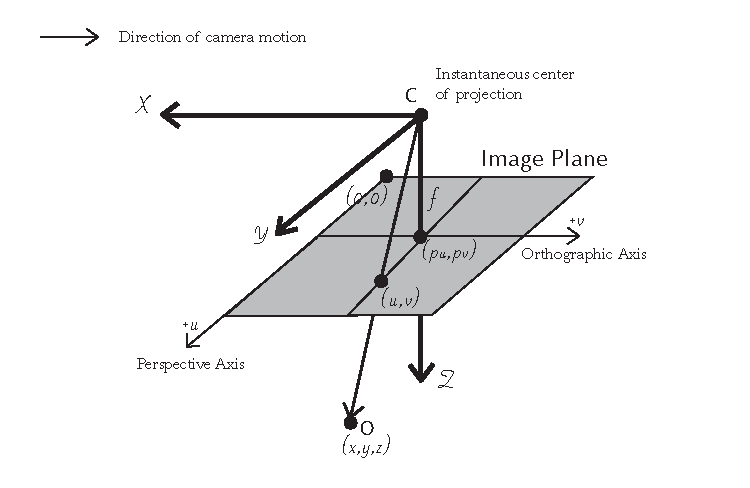
\includegraphics[width=6in]{images/linescan_geometry.pdf}
 \end{center}
  \caption{Geometry of the Linescan Camera Model.}
  \label{fig:linescan-geometry}
\end{figure}

The geometry of the linescan imager is subtly different from the
geometry of the pinhole camera.  See Figure
\ref{fig:linescan-geometry}.  Although there is still a center of
projection created by the camera's optics (and points are still imaged
using a perspective projection in the across-track direction), this
point moves as the camera moves, and as a result, the along-track
position of a pixel in a linescan image is purely a function of the
position and orientation of the camera; both a function of time.  The
orientation of the image (in the sense that $u$ indexes the columns of
an image and $v$ indexes its rows) must be chosen consistent with
Figure \ref{fig:linescan-geometry} when working with
\verb#LinescanModel# and its relatives.

In the special case where the motion of the linescan sensor is linear
and its orientation is fixed, the projection of the points onto the
image in the along-track direction is orthographic.  These assumptions
are the basis for the {\em Linear Pushbroom Model}, which can be found
in the header file \verb#<vw/Camera/LinearPushbroomModel.h>#.  If you
are interested in understanding this model in detail, we recommend you
read the excellent paper by Gupta and Hartly \cite{gupta97}.

If you must relax the assumption about a linear flight path somewhat
to allow sensor pose to vary and the camera motion to lie along a
curve (as is common with orbiting camera systems), the {\em Orbiting
  Pushbroom Model} is an appropriate choice.  In the Orbiting
Pushbroom model, the user supplies a series of evenly spaced samples
of position and orientation and specifies the time interval (in
seconds) between samples.  A sparse set of samples is sufficient for
this model: interpolation occurs for points in between the supplied
positions and orientations.

\section{Tools for Working With Camera Images}

This section describes several tools that simplify the process of
working with image captured by real cameras.

\subsection{Inverse Bayer Pattern Filtering}

Most imaging sensors are inherently grayscale capture devices.  In
order to capture color, some imagers have a hardware color filter
placed in front of the pixels on the CCD.  This is called a 
{\em Bayer filter}.  The Vision Workbench provides the
\verb#inverse_bayer_filter()# function (found in the header file
\verb#<vw/Camera/BayerFilter.h>#) which interprets the raw, grayscale
pixel values from the sensor and produces a color image by
interpreting the Bayer filter effect.

\subsection{Exif Exposure Data}

Digital cameras store data about the settings used to take a picture
in the image file according to the EXIF standard \cite{exif}. EXIF
data is stored using the Image File Directory system described in the
TIFF 6.0 standard.  EXIF tags such as {\tt FNumber} and
{\tt ExposureTime} can be useful for radiometrically calibrating your
camera images.  Unfortunately the standard is redundant and often
poorly supported by camera manufacturers (for example, many hide the
ISO setting in the maker note instead of storing it in the
ISOSpeedRatings tag), so we cannot guarantee support for every camera.

The Camera module includes the {\tt ExifView} class (defined in
\verb#<vw/Camera/Exif.h>#) for extracting this data from images.  To
create this class, you supply the filename of an image on disk.
Currently, JPEG and TIFF images are supported.  ExifData and ExifView
were based on {\tt jhead}, an EXIF JPEG header and thumbnail manipulator
program in the public domain \cite{jhead}.

\begin{verbatim}
  // Reliably get F number. 
  ExifView view;
  if (view.load_exif(``img.jpg'')) {
    double f = view.get_f_number();
    // ...
  }
\end{verbatim}

\begin{thebibliography}{1}

\bibitem{exif} ``Exchangeable image file format for digital still cameras: Exif Version 2.2'',
(Japan Electronics and Information Technology Industries Association, 2002),
http://www.exif.org/specifications.html.

\bibitem{gupta97} Gupta, Rajiv and Hartley, Richard. ``Linear Pushbroom Cameras''.  IEEE
 Transactions on Pattern Analysis and Machine Intelligence. Vol.19 No. 9. September 1997

\bibitem{jhead} Wandel, Matthias, ``Exif Jpeg header and thumbnail manipulator program,'' 2006,
http://www.sentex.net/~mwandel/jhead/.

\bibitem{yakimovsky78}  Yakimovsky, Y. and Cunningham R., ``A System for Extracting
  Three-Dimensional Measurements from a Stereo Pair of TV Cameras ''
  Computer Graphics and Image Processing 7, pp. 195-210. (1978)

\end{thebibliography}

\chapter{The {\tt Mosaic} Module}\label{ch:mosaic-module}

The \verb#Mosaic# module provides a number of tools for assembling and
generating image mosaics, i.e. large images that are composed of a
number of smaller images.  The applications of this module include
panoramic imaging and aerial/satellite image processing.  There are 
three major facilities provided at this time: compositing many images 
together, using multi-band blending to seamlessly merge overlapping 
images, and generating on-disk image quadtrees to efficiently store 
very large images.

Note that the facilities described in this chapter are currently under
active development, and there may be some API changes in future
releases as new capabilities are added.

\section{{\tt ImageComposite} and Multi-Band Blending}\label{sec:imagecomposite}

The \verb#ImageComposite# template class provides the ability to
composite any number of source images together at arbitrary pixel
offsets.  It was originally designed for assembling tiled panoramas or
aerial/satelite images that have been transformed into a common
coordinate system, though it could be used for many other things as
well.

The main interface is fairly simple.  Just like ordinary Vision
Workbench images, an \verb#ImageComposite# is templatized on its pixel
type.  In most cases you will want to use a pixel type that has an
alpha channel, and if you want to perform image blending then the
pixel type must be floating-point, so the most common pixel type is
\verb#PixelRGBA<float32>#.  You can then configure whether you would 
like to use multi-band blending to merge your images or if you would 
simply like them overlayed by using the \verb#set_draft_mode()# 
method.  It takes a single argument which sould be \verb#true# if 
you simply want to overlay the images and \verb#fales# if you want 
to use the blender.  Blending is a significantly more expensive 
operation.  If your images do not overlap but are simply tiles then 
draft mode is probably what you want. 

Once you have created the composite object, you add source images to
it using the \verb#insert()# method, which takes three arguments: the
image you are adding, and the $x$ and $y$ pixel offset of that image
within the composite.  The \verb#ImageComposite# does not store a copy
of your image.  Instead, it only stores a reference to it in the form
of an \verb#ImageViewRef# object.  This means that you can easily do
things like create a composite of images that could not all fit in
memory simultaneously, e.g. by passing in \verb#DiskImageView#
objects.  Note that only integer pixel offsets are supported: if you
want to shift an image by a fractional amount you will first need to
transform it accordingly.  In most cases you will need to
pre-transform your source images anyway, so this applies no extra
cost.

Once you have added all your images, be sure to call the 
\verb#ImageComposite#'s \verb#prepare()# method.  This method takes 
no arguments, but it does two things.  First, it computes the 
overall bounding box of the images that you have supplied, and 
shifts the coordinate system so that the minimum pixel location 
is $(0,0)$ as usual.  Second, if multi-band blending is enabled, 
it generates a series of mask images that are used by the blender. 
Currently these are saved as files in the current working directory. 
This is admittedly inconvenient behavior and will be changed in a 
future release.

Now that you've assembled and prepared your composite you can use 
it just like an ordinary image, except that per-pixel access is 
not supported.  If the image is reasonably small then you can 
rasterize the entire image by assigning it to an \verb#ImageView#. 
Alternatively, if the composite is huge the usual next step is to 
pass it as the source image to the quad-tree generator, discussed 
in the next section.  You can also use \verb#ImageComposite#'s 
special \verb#generate_patch()# method to manually extract smaller 
regions one at a time.  It takes a single \verb#BBox2i# bounding-box, 
expressed in the re-centered coordinate frame, as its only argument.

Here's a simple example that illustrates how you might blend 
together a number of images on-disk.  It assumes you already know 
the image filenames and their offets within the commposite, and 
that the total composite is small enough to sensible rasterize all 
at once.
\begin{verbatim}
ImageComposite<PixelRGBA<float> > composite;
for( int i=0; i<num_images; ++i ) {
  composite.insert( DiskImageView<PixelRGBA<float> >( image_filename[i] ),
                    image_offset[i].x(), image_offset[i].y() );
}
composite.prepare();
write_image( "composite.png", composite );
\end{verbatim}
For a somewhat more fleshed-out example of how to blend images, 
see the example program \verb#blend.cc# included with the 
\verb#Mosaic# module sources.

\begin{figure}[t]
\centering
  \subfigure[First source]{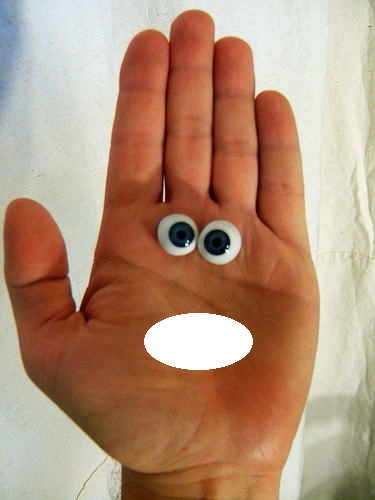
\includegraphics[width=2in]{images/hand.jpg}\label{fig:blend.hand}}
  \hfil
  \subfigure[Second source]{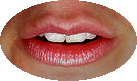
\includegraphics[width=1.23in,trim = -0.5in -1.5in -0.5in 0in]{images/lips.jpg}\label{fig:blend.lips}}
  \hfil
  \subfigure[Blended result]{\includegraphics[width=2in]{images/hand-lips-blend.jpg}\label{fig:blend.result}}
\caption{Example input and output images from the {\tt ImageComposite} multi-band 
blender.\protect\footnotemark }
\label{fig:blend.hand}
\end{figure}
\footnotetext{Original hand and face source images by {\tt sheldonschwartz} and {\tt vidrio}, respectively, and released under the Creative Commons license.}

\begin{figure}[p]
\centering
  \subfigure[Draft mode (simple overlay)]{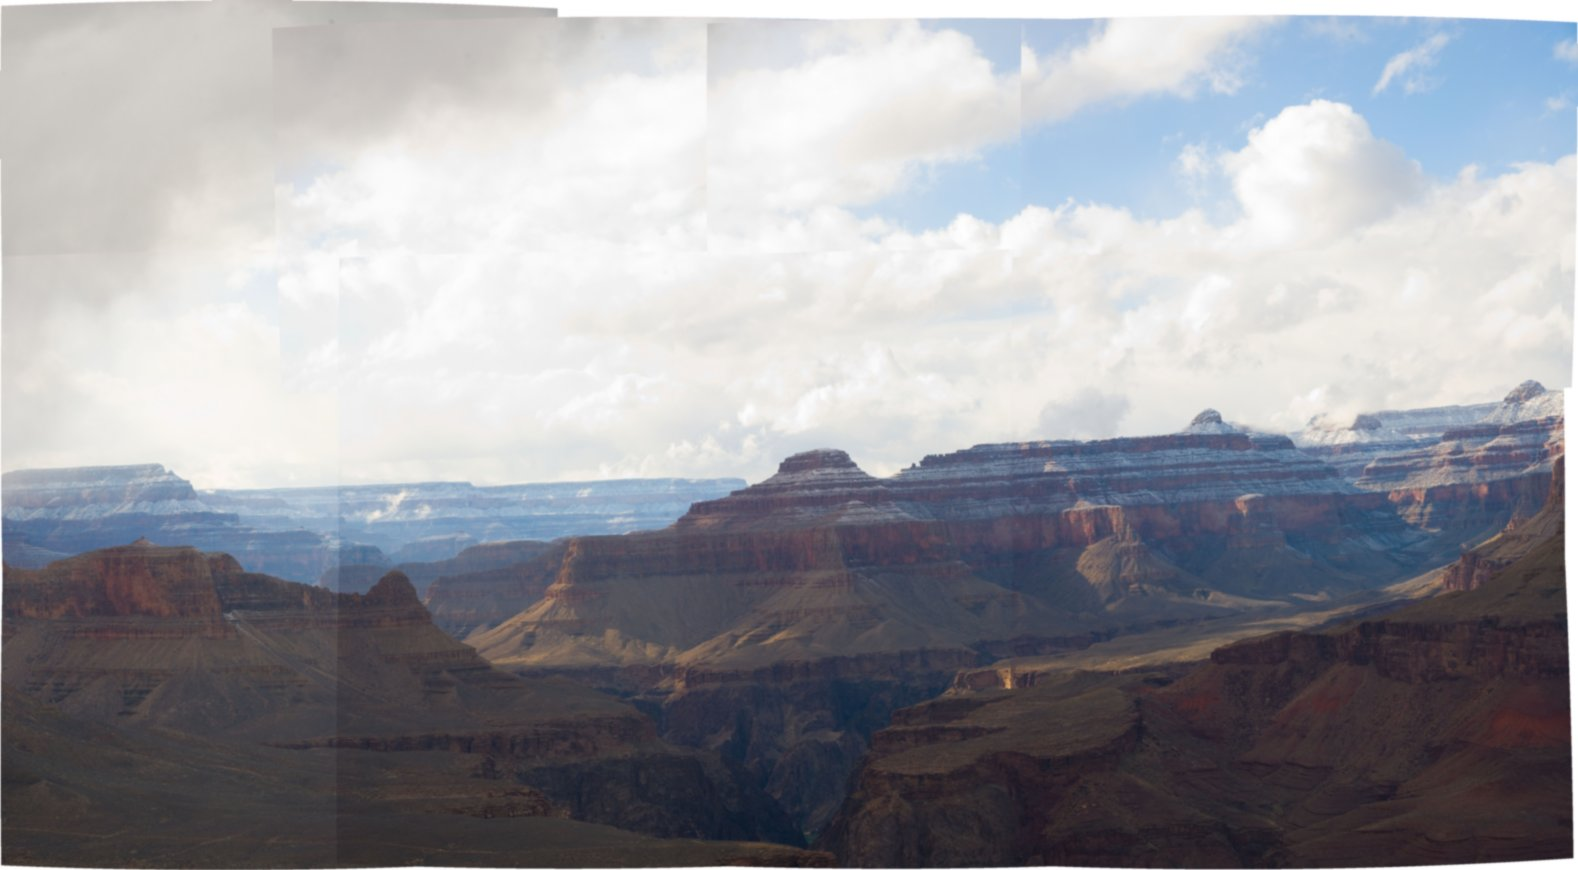
\includegraphics[width=6.5in]{images/kiabab-draft.jpg}\label{fig:kiabab.draft}}
  \\
  \subfigure[Multi-band blending]{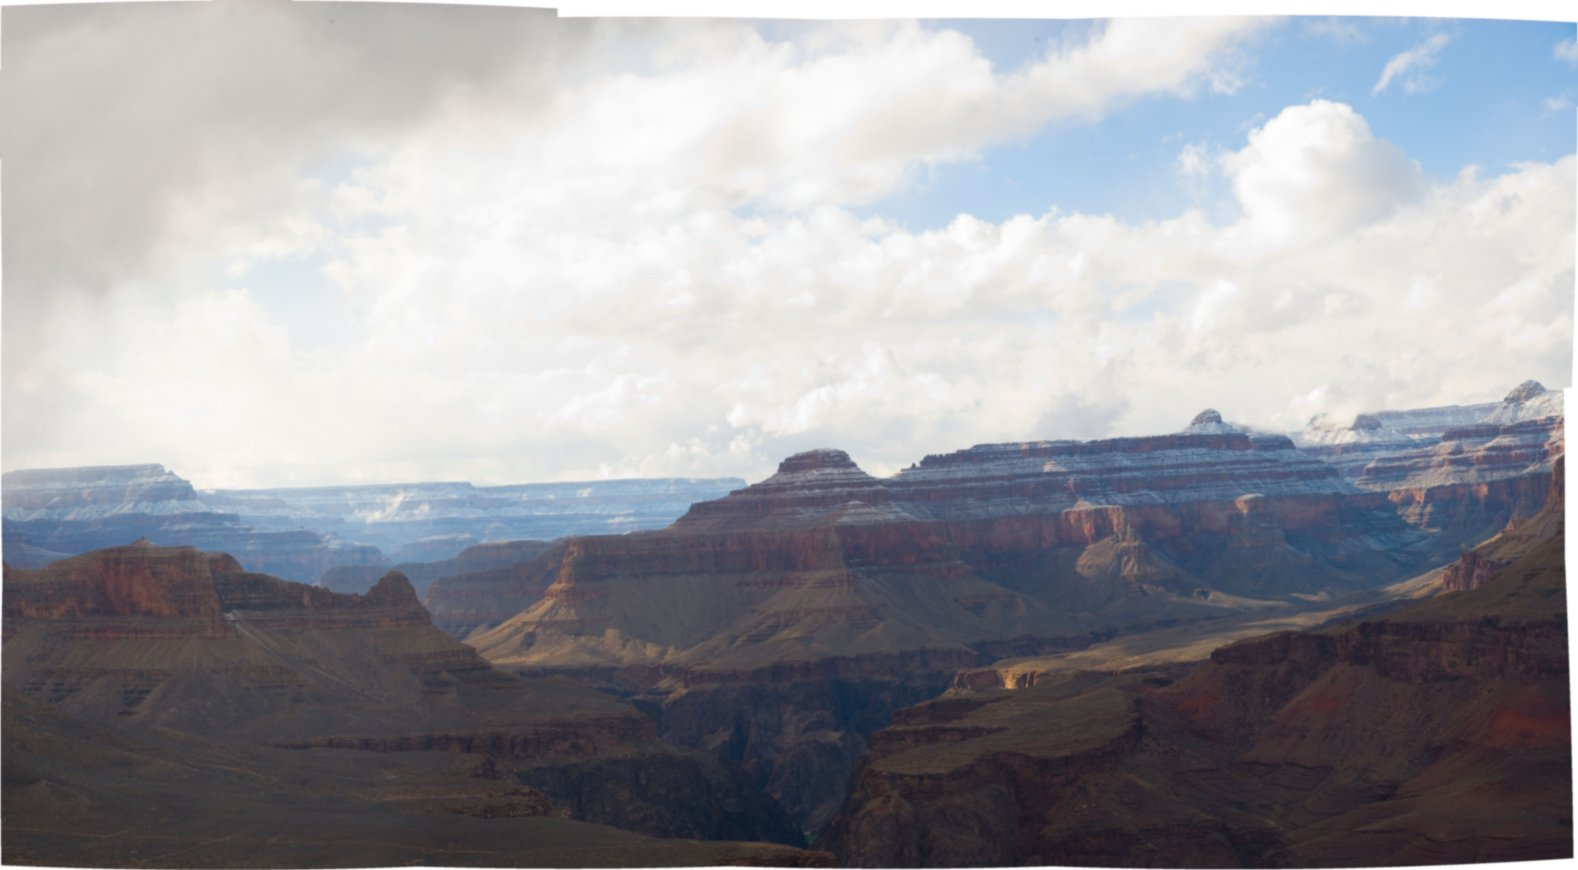
\includegraphics[width=6.5in]{images/kiabab-blend.jpg}\label{fig:kiabab.blend}}
\caption{A twelve-image mosaic composited using an {\tt ImageMosaic} object, first in 
draft mode (a) and then musing multi-band blending (b).}
\label{fig:blend.kiabab}
\end{figure}

\section{{\tt ImageQuadTreeGenerator}}\label{sec:quadtreegenerator}

The ability to assemble composites that are far larger than could be stored 
in memory all at once presents serious challenges.  When viewing an image 
of that size, the ability to zoom in and out is of critical importance.  
Only a small fraction of the image data will ever be on-screen at a time 
at full resolution.  However the entire data set may be visible at once at 
lower resolutions, and computing such reduced images on the fly can be 
prohibitively expensive.  The usual solution to this problem is to 
pre-compute subsampled versions of the image at multiple levels of detail. 
The subsampling factors are often chosen to be successive powers of two, 
and the data at each resolution is typically chopped up into tiles for 
faster direct access.

The \verb#ImageQuadTreeGenerator# class generates just such a representation 
of an image.  You specify the tile size, the generator reduces the 
image by powers of two until it fits in a single tile.  To generate 
each successive level of detail every tile is replaced by four tiles 
at twice the resolution.  The resulting quad-tree of images is stored 
on disk in a hierarchical manner, making it easy to instantly access any 
tile at any resolution.

Like most everything else in the Vision Workbench, a \verb#ImageQuadTreeGenerator# 
is templatized on its pixel type.  The constructor takes two arguments, 
the pathname of the tree to be created on disk and the source image. 
You can then use several member functions to configure the quad-tree 
prior to generating it.  The \verb#set_bbox()# method, which takes a 
single \verb#BBox2i# parameter, specifyies that a particular region of 
the source image to be processed instead of the entire thing.  The 
\verb#set_output_image_file_type()# method sets the file type of the 
generated image files; the default is ``\verb#png#''.  The 
\verb#set_patch_size()# function takes an integer argument specifying 
the patch size in pixels.  Relatedly, the \verb#set_patch_overlap()# 
function specifies how many pixels of the border of each patch overlap 
the neighboring patch.  The default is $256$-pixel patches with no 
overlap.  Finally, the \verb#set_crop_images()# method takes a 
boolean argument that controls whether or not the resulting images 
are cropped to the non-transparent region.  Image cropping is enabled 
by default.

Once you have configured the \verb#ImageQuadTreeGenerator# to your liking
you can invoke its \verb#generate()# method to generate the quad-tree
on disk.  It is stored in a directory with the name you provided as
the first argument to the constructor with the extension
``\verb#.qtree#'' appended.  For example, if you specified the name of
the quad-tree as \verb#/home/mdh/example# then the result is stored in
the directory \verb#/home/mdh/example.qtree#.  This directory
typically contains three things.  First is the lowest-resolution image
of the tree, essentially a thumbnail, which is stored in an image with
the same base name as the tree with the appropriate image file format 
extension appended.  To continue the above example, if the file format 
type is ``\verb#png#'' then the top-level image file's pathname will be 
\verb#/home/mdh/example.qtree/example.png#.  The next file in the 
top-level directory is a simple text file describing the bounding box 
of the top-level patch, with the same name but with the extension 
\verb#.bbx# instead.  The format of this file will be discussed below.  
Finally there is a subdirectory, which has the same name but no extension,
that contains the next level of the tree.

Inside that subdirectory there are generally four image files, with
names \verb#0.png#, \verb#1.png#, \verb#2.png#, and \verb#3.png#,
containing to the four image patches at the second level of
detail. The patches are numbered left-to-right and top-to-bottom, so
\verb#0# is the upper-left patch, \verb#1# is the upper-right patch,
and so on.  There are also four corresponding \verb#.bbx# files and
four directories containing higher-resolution data for each patch.
Each subdirectory likewise has four numbered images, bounding boxes,
and further subdirectories.  For example, the file
\verb#/foo/bar/myimage.qtree/myimage/0/1/3.png# would be an image at
the fourth level of detail.  The subdirectories at the highest level
of detail have no further subdirectories.  Note that if cropping is
enabled then it is possible that some directories will not have all
four images; this occurs if any of the images is entirely empty.

Each \verb#.bbx# file contains eleven numbers, represented as test
strings, each on a line by itself.  The first is the scale factor of
that tile: it has the value $1$ for the highest-resolution patches and
values of the form $2^n$ for lower-resolution patches.  You can
equivalently think of this number as describing the size of each pixel
at this resolution, as measured in full-resolution pixels.  The next
four numbers describe the bounding box of the patch within the
full-resolution coordinate system.  First are the $x$ and $y$
coordinates of the upper-left pixel, and then come the width and
height of the image in pixels.  To reiterate, these are measured in
{\it full-resolution} pixels, and so these numbers will generally be
multiples of the scale factor.

After this come a similar set of four numbers describing the bounding
box of the unique image data in this patch.  This is generally the
same as the previous bounding box if there is no patch overlap.
However, if the patch overlap has been set to a nonzero value then
this second bounding box will describe the portion of this patch that
does not overlap the corresponding regions of the neighboring patches.
In other words, taken together these second bounding boxes perfectly
tile the entire image without overlap.  Finally, the last two values
describe the width and height of the entire source image in pixels.

This file format is obviously quite arbitrary.  In a future release 
we hope to provide hooks to allow the user to specify their own 
meta-data formats, and we may change the default format to something 
more flexible.

\begin{figure}[t]
\centering
  \subfigure{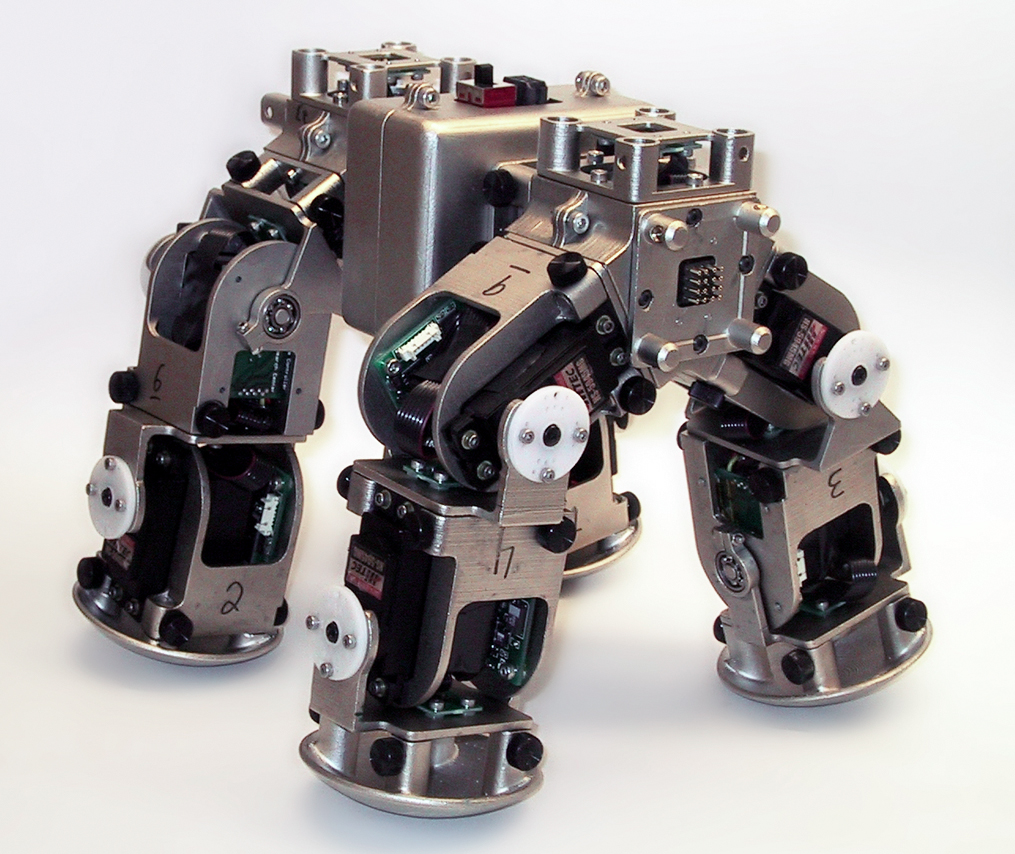
\includegraphics[height=1.5in]{images/Walker.qtree/Walker.jpg}\label{fig:walker.a}}
  \hfil
  \subfigure{\includegraphics[height=1.5in]{images/Walker.qtree/Walker/1.jpg}\label{fig:walker.b}}
  \hfil
  \subfigure{\includegraphics[height=1.5in]{images/Walker.qtree/Walker/1/2.jpg}\label{fig:walker.c}}
\caption{Patches at three successive resolutions generated by an {\tt ImageQuadTreeGenerator} 
constructed with the name ``{\tt Walker}''.  The files are named {\tt Walker.qtree/Walker.png}, 
{\tt Walker.qtree/Walker/1.png}, and {\tt Walker.qtree/Walker/1/2.png}, respectively.}
\label{fig:blend}
\end{figure}

\chapter{High Dynamic Range Imaging}\label{ch:hdr-imaging}

Photographers have long understood that the range of brightness levels in
a real-world scene is considerably larger than the range that can be
captured by a camera's film or imaging sensor.  The luminance of a
outdoor scene can easily span five orders of magnitude, however
typical digital cameras encode the brightness at a single pixel
location using a modest 8-bits (2 orders of magnitude).  Pixels that
fall outside the {\em dynamic range} of the camera sensor will either
be underexposed or overexposed; their values will be at the minimum or
maximum pixel value of the camera, respectively.

Some digital cameras can save RAW images with higher dynamic range
than normal.  These cameras can capture 12 bits per pixel, or 4096
brightness levels.  This expanded dynamic range is often sufficient to
capture scenes with a moderate amount of contrast. To capture scenes
with very high dynamic range you can generate an HDR image from a set
of {\em bracketed} exposures: a group of low dynamic range images of
the exact same scene taken with a set of different exposure settings
that varies from under-exposed to over-exposed.  This technique is
subject of section \ref{sec:hdr_merge}.

The resulting HDR image is generally stored with a channel type of
{\tt float} or {\tt int16} to accomodate the expanded dynamic range.
To store HDR images on disk we recommend using the OpenEXR or TIFF
file formats, both of which support 32-bit floating point channel
types.

Just as capturing HDR images can be challenging, visualizing them is
also difficult.  Print media and most display devices can only manage
about 2 orders of magnitude of dynamic range, whereas an HDR image may
have 5 or more orders of magnitude. Simply scaling the image to the
display range will cause it to look overly dark or washed-out. Section
\ref{sec:tonemapping} discusses a technique called {\em tone mapping}
that reduces the dynamic range of an image while preserving as much as
possible the visual contrasts of the original scene.

\section{Merging Bracketed Exposures}
\label{sec:hdr_merge}

As discussed in the introduction to this chapter, the limited dynamic
range of the sensors on modern cameras necessitates a different
strategy for building true HDR images: exposure backeting.  This frees
us from hardware limitations and allows us to set the dynamic range of
the output image by adjusting the range of exposures in the bracket.
If more dynamic range is needed, one can simply add additional
exposures on either side of the bracket.

\begin{figure}[tbp]
\begin{center}
  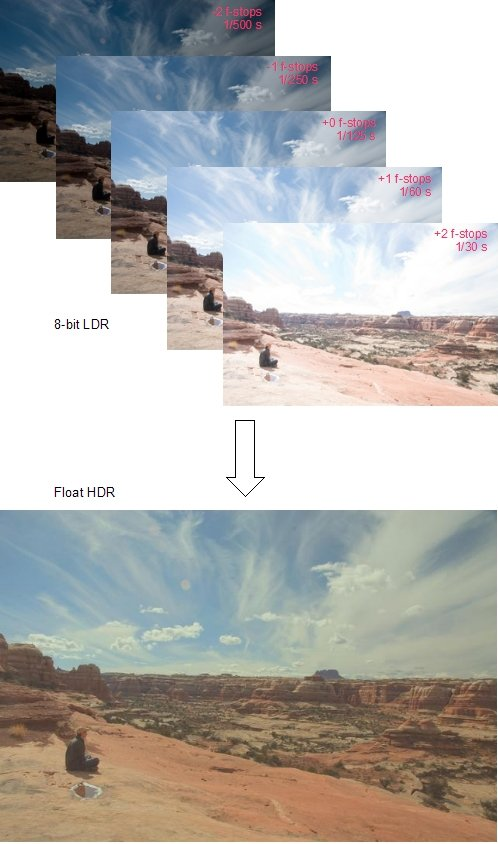
\includegraphics[width=5in]{images/hdr_merge.jpg}
 \end{center}
  \label{fig:hdrmerge}
  \caption{A stack of 8-bit-per-channel LDR images separated by one
    f-stop is merged a floating-point HDR image. The HDR image is
    tone-mapped for display using the Drago operator.}
\end{figure}

For convenience, the exposure ratio between consecutive images is
usually fixed {\em a priori} to guarantee a wide exposure range while
maintaning even brightness overlap between adjacent images in the
bracket. A factor of two is generally recommended.  The shutter speed
is generally the preferred method of varying the exposure in a
bracket; changing the aperture or ISO setting can have the same effect
on exposure but they may change the focus or increase noise.

\subsection{Using HDR Stacks}
The HDR module has a set of free functions that make stitching a stack of LDR
images into an HDR image as simple as one function call. process\_ldr\_images (in 
LDRtoHDR.h) takes a std::vector of ImageViews (with grayscale or RGB pixels
and a floating point channel type), sorted from darkest to brightest. This
function assumes a constant exposure ratio between images; it can be specified
or the default of $\sqrt{2}$ can be used for stacks with a ratio of 1 EV. An
overloaded version also accepts a std::vector$<$vw::Vector$<$double$>$ $>$ by reference,
to return the estimated response curves for each channel.

\begin{verbatim}
/* Generate HDR image from HDR stack. */
typedef ImageView<PixelRGB<double> > Image;
vector<Image> images(num_images);
// ... Read input images ...
// Assume default exposure ratio.
Image hdr_image = process_ldr_images(images);
\end{verbatim}

LDRtoHDRExif.h further defines process\_ldr\_images\_exif, which generates an HDR
image from an array of filenames of LDR images, computing brightness values
from the files' Exif data. Example code usingthis function is in Appendix B. It
also defines another overloaded version of process\_ldr\_images that takes a
std::vector$<$double$>$ of brightness values (as defined by the APEX system \cite{apex})
instead of a constant exposure ratio. These functions do not require the images
to be in any particular order of have a constant exposure ratio.

\subsection{Alignment}
It is crucial for the images in an HDR stack to be aligned, both so
that the resulting HDR image is not blurry and so that the camera
response curve can be estimated accurately.  The best solution is to
take the HDR stack on a tripod, ideally using remote capture.  {\em If
  you are able to take the images on a stationary platform, there is
  no need to perform image alignment in software.}  However, for
handheld photographs, or if dynamic disturbances, such as wind, shake
the camera on the tripod, software alignment is then likely to be
necessary.

For HDR stacks shot with a hand-held camera or otherwise unaligned,
the HDR module includes MTBAlign.h, an implementation of the Mean
Threshold Bitmap (although it actually uses the median) alignment
technique \cite{hdrbook}. MTB alignment thresholds two images on their
respective medians and finds the x- and y-shifts that minimize the
difference of the resulting bitmaps. This technique is well-suited for
HDR stacks as the median threshold bitmap is relatively invariant with
respect to the exposure used to take the photo, whereas edges may fade
in and out. The weakness of MTB alignment is that it only considers
translation. This should be sufficient even for most photos taken
hand-held, but to align images that are rotated or otherwise warped, a
more sophisticated alignment technique should be used (the
InterestPoint module, for example).

\begin{verbatim}
// Find the shift to be applied to img2 to match it most
// closely with img1.

int shift_bits = 6; // Maximum shift of 64 pixels
int shift[2];       // Will hold (x,y) shift

// img1 and img2 assumed to be of type
// ImageView<PixelGray<double> >.
get_exp_shift(img1, img2, shift_bits, shift);
\end{verbatim}

\subsection{Camera Response Curves}
The relation between light entering a camera sensor and the pixel
value that is ultimately recorded is non-linear.  The function that
maps the amount of light on the sensor (the luminance) to the pixel
value is referred to as the camera response curve.  [TODO: Add camera
  response curve figure.]  

\begin{figure}[tbp]
\begin{center}
  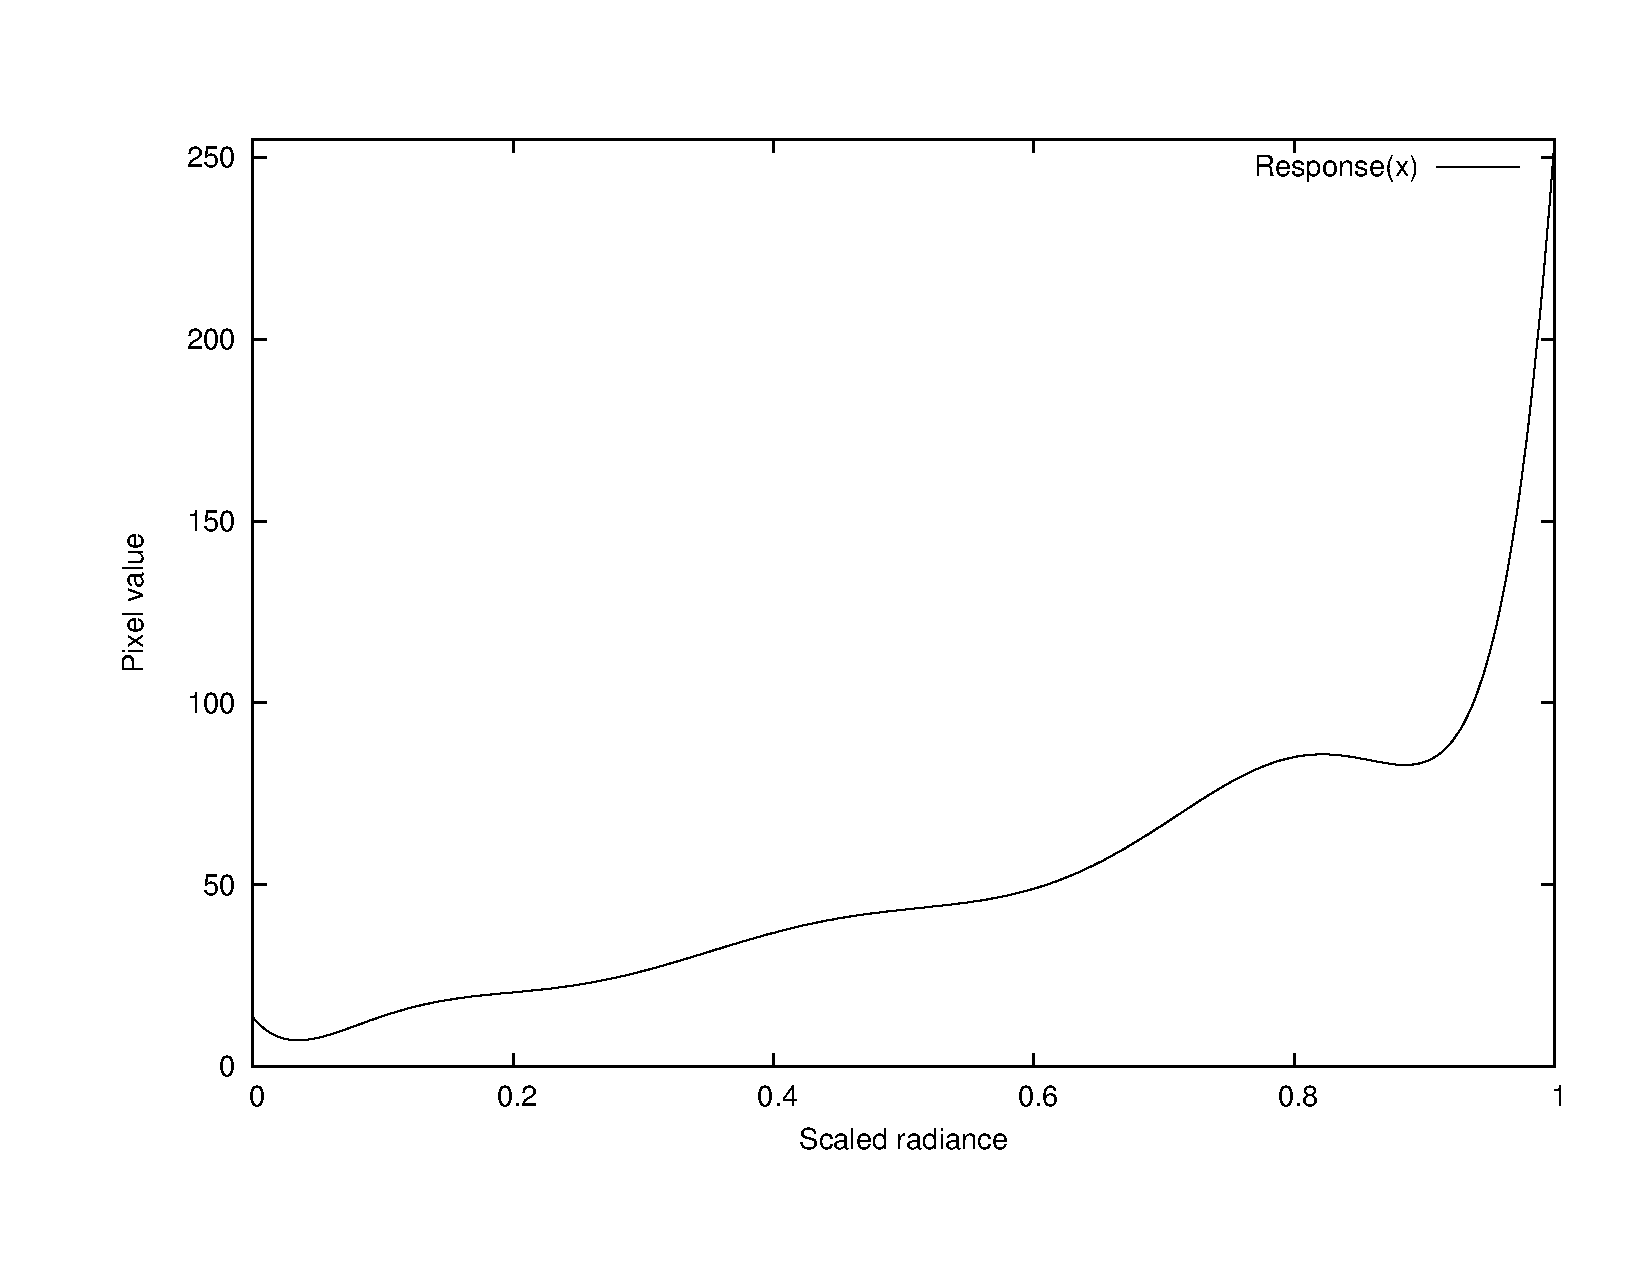
\includegraphics[width=5in]{images/hdr_response.pdf}
 \end{center}
  \label{fig:response}
  \caption{Camera response curve estimated from an HDR stack.}
\end{figure}

To create an HDR image that truly represent the physical brightness
levels in a scene, it is necessary to estimate the inverse of the
camera response curves (we assume a separate curve for each channel)
and apply it to the image data.  That is, we would like to find a
function that, given a pixel value in the image and its exposure
information, returns the luminance of the scene at that point.
CameraCurve.h and CameraCurve.cc implement {\tt
  estimate\_camera\_curve()}, a free function that estimates the
inverse response curve as a polynomial.  This routine takes a matrix
of aligned pixel channel values from an HDR stack and their brightness
ratios. This function is used by LDRtoHDR.h and its relatives; most
users will probably not need to call it directly.

The CameraCurve sources also supply {\tt invert\_curve()}, a free
function that approximates the inverse of a polynomial curve, also as
a polynomial. This is useful to recover the actual camera response
curve (mapping a scaled luminance value to a pixel value) from the
inverse response curve determined by {\t
  estimate\_camera\_curve()}. Re-applying the camera response curve to
an HDR image after tone-mapping can improve the colors and overall
visual appeal. See the code example in Appendix B for an example.

\section{Tone Mapping}
\label{sec:tonemapping}
Since print media and most display technologies are inherently LDR,
an the dynamic range of an HDR image must be compressed before it
can be displayed. Simply scaling the pixel luminances linearly
yields poor results because the human visual system's response to
luminance is approximately logarithmic rather than linear. A linear
scaling tends to lose small details and local contrast, and the
image as a whole will appear under- or over-exposed.

A wide variety of tone-mapping operators have been proposed to
compress the dynamic range of an HDR image while preserving
details and local contrast as much as possible. Using an ideal
tone-mapping operator, the observer of a tone-mapped LDR image
would have a perceptual response matching that of the original
HDR scene. Due to its greater realism, tone-mapping generally
vastly improves the appearance of the displayed image.

There are several broad classes of tone-mapping operators, including
global operators, local operators, and operators that use the
gradient or frequency domains. The HDR module currently includes
one global operator and one local operator; they are described in
the following sections.

\subsection{Global Operators}
Global tone-mapping operators apply the same compressive function to
all pixels in the image. Such operators are implemented in
GlobalToneMap.h/.cc. Currently one such operator is implemented, the
Drago Adaptive Logarithmic Mapping operator.  For algorithm details
see \emph{High Dynamic Range Imaging} \cite{hdrbook} or the original
paper \cite{drago}.  The Drago operator is currently the operator of
choice in the HDR module. It is quite fast, produces good results for
a wide range of images, and can usually be used with its parameters at
default values. Optionally, the parameters bias (controlling contrast,
usually between 0.7 and 0.9), exposure factor (a simple multiplier to
control the overall brightness of the image), and max display
luminance (usually about 100) can be specified.

\begin{verbatim}
/* Apply Drago tone-mapping operator */
ImageView<PixelRGB<float> > tone_mapped = drago_tone_map(hdr_image);
\end{verbatim}

\begin{figure}[tbp]
\begin{center}
  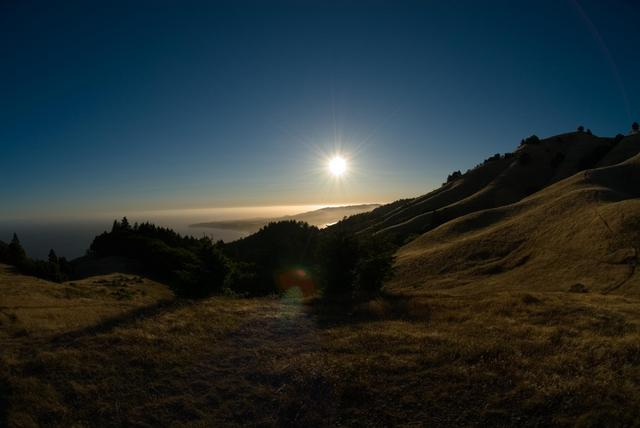
\includegraphics[height=3in]{images/hdr_original.jpg}
  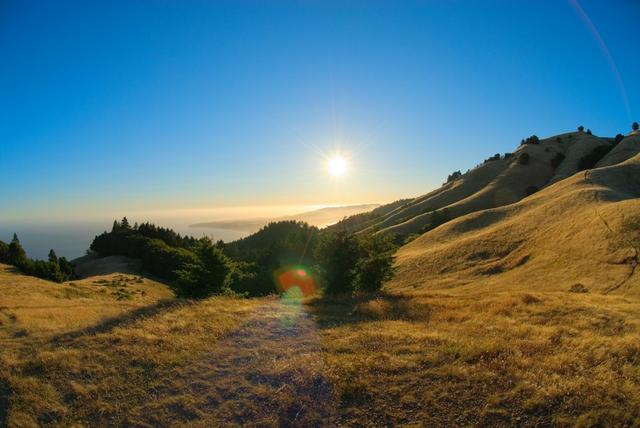
\includegraphics[height=3in]{images/hdr_drago.jpg}
  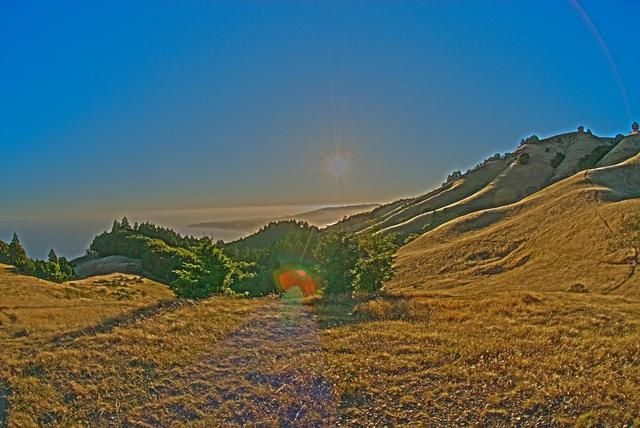
\includegraphics[height=3in]{images/hdr_ashikhmin.jpg}
 \end{center}
  \label{fig:tonemapping}
  \caption{Top: an image taken in 12-bit RAW format. Middle: after
           tone-mapping with the Drago operator. Bottom: after
           tone-mapping with the Ashikhmin operator.}
\end{figure}

\subsection{Local Operators}
Local tone-mapping operators compress a pixel's dynamic range in a way
dependent on the neighborhood of pixels around it. These operators
mimic the local adaptation of the human eye and are capable of more
striking or artistic results than global operators, but they are also
susceptible to artifacts such as excessive haloing and reverse
gradients. LocalToneMap.h/.cc currently implements the Ashikhmin local
tone-mapping operator \cite{ashikhmin}.  It is much slower than the
Drago operator and more prone to artifacts, but may be useful for some
images. Its only parameter is a threshold value (0.5 by default) which
roughly controls the size of the neighborhood used for each pixel. A
threshold value too large will result in haloing.

\begin{verbatim}
/* Apply Ashikhmin tone-mapping operator */
ImageView<PixelRGB<float> > tone_mapped = ashikhmin_tone_map(hdr_image);
\end{verbatim}

\subsection{Using HDR Stacks}
The HDR module has a set of free functions that make stitching a stack of LDR
images into an HDR image as simple as one function call. process\_ldr\_images (in 
LDRtoHDR.h) takes a std::vector of ImageViews (with grayscale or RGB pixels
and a floating point channel type), sorted from darkest to brightest. This
function assumes a constant exposure ratio between images; it can be specified
or the default of $\sqrt{2}$ can be used for stacks with a ratio of 1 EV. An
overloaded version also accepts a std::vector$<$vw::Vector$<$double$>$ $>$ by reference,
to return the estimated response curves for each channel.

\begin{verbatim}
/* Generate HDR image from HDR stack. */
typedef ImageView<PixelRGB<double> > Image;
vector<Image> images(num_images);
// ... Read input images ...
// Assume default exposure ratio.
Image hdr_image = process_ldr_images(images);
\end{verbatim}

LDRtoHDRExif.h further defines process\_ldr\_images\_exif, which generates an HDR
image from an array of filenames of LDR images, computing brightness values
from the files' Exif data. Example code usingthis function is in Appendix B. It
also defines another overloaded version of process\_ldr\_images that takes a
std::vector$<$double$>$ of brightness values (as defined by the APEX system \cite{apex})
instead of a constant exposure ratio. These functions do not require the images
to be in any particular order of have a constant exposure ratio.

\section{Panoramic HDR}
Applying HDR techniques to panoramic images is extremely challenging,
as it is necessary to consider how each individual image is placed in
the full panorama.  LDRtoHDRPano.h contains prototype code for
computing the response curves from a set of panoramic images and
projecting the individual images into the same luminance
space. Blending the resulting images together into a full panorama is
left to a separate blender.

The difficult part is computing the camera response curves from the
panoramic images; it would be simpler to compute and cache the
response curves using a standard HDR stack, but on digital cameras the
response curves may vary with settings. Basically, the areas of the
panorama where two or more individual images overlap are used as HDR
stacks for sampling. The panorama is traversed considering one square
section at a time, so that only those images overlapping that section
need to be loaded (keeping all of the individual images in memory at
once would be too memory-inefficient).  Brightness data is extracted
from the Exif data in the original images.

LDRtoHDRPano.h defines the free function
process\_ldr\_images\_pano. The inputs will likely need to be changed
to accept whatever variety of ImageView(Ref) the panorama alignment
algorithm produces. Currently the inputs are a vector of PanoImage
structs, an optional vector of brightness values for the images
(otherwise Exif is used), the width and height of the full panorama,
and a vector of vw::Vectors to store the computed camera response
curves. PanoImage holds the image's file name, a Rect struct which
holds its dimensions and offset within the panorama, and a
brightness\_multiplier field in which process\_ldr\_images\_pano
stores a multiplier that will project the image into the same
luminance space as the others (after applying the camera curves using
the function psi from LDRtoHDR.h). The outputs are the camera response
curves and the brightness multipliers.

\section{Command Line Utilities}
There are a number of freely available command line utilities which are useful for working
with HDR images. The OpenEXR distribution \cite{openexr} includes several utilities,
including exrdisplay for displaying OpenEXR images. exrtools \cite{exrtools} provides
utilities for converting between OpenEXR and other formats, performing basic operations
on OpenEXR images, and a couple of tone-mapping utilities. pfstools \cite{pfstools} is a
well-integrated set of utilities for reading, writing, manipulating and viewing HDR images.
It has an associated pfstmo project that implements seven of the more prominent tone
mapping operators.

\begin{verbatim}
/* Create a PanoImage struct */
PanoImage img = PanoImage(``img.jpg'', Rect(img_x,
                img_y, width, height), 0);

/* Compute response curves and brightness multipliers */
vector<PanoImage> images;
vector<Vector<double> > curves;
// ... load images ..
process_ldr_images_pano(images, pano_width,
                        pano_height, curves);
\end{verbatim}

\section{List of Files}
\begin{description}
\item[CameraCurve.h, cc] Functions for estimating camera response curves and inverting curves.
\item[ExifData.h, cc] Class for reading Exif data from JPEG or TIFF images. Offers access to
any tag referenced by tag ID.
\item[ExifView.h, cc] Class providing a convenient interface for extracting exposure data
from Exif.
\item[GlobalToneMap.h, cc] Functions for applying global tone-mapping operators. Currently
implements the Drago operator.
\item[GradientDomain.h, cc] Functions for applying gradient domain tone-mapping operator.
Currently implements the Fattal operator.
\item[LDRtoHDR.h] Functions for generating an HDR image from an HDR stack of LDR images
using either a constant exposure ratio.
\item[LDRtoHDRExif.h] Extends functionality of LDRtoHDR.h to use exposure data from Exif.
\item[LDRtoHDRPano.h] Estimates response curves and brightness multipliers for aligned
images in a panorama.
\item[LocalToneMap.h, cc] Functions for applying local tone-mapping operators. Currently
implements the Ashikhmin operator.
\item[print\_exif.cc] An example program which uses ExifView to display some Exif data.
\end{description}

\section{Full Code Example}
\begin{verbatim}
/* ExifHDR_test.cc
 * 
 * This is a simple test program that stitches an
 * Exif-tagged HDR stack into an HDR image,
 * performs tone-mapping, and saves several
 * versions with different post-processing applied
 * for comparison. Usually the best image is
 * produced by re-applying the camera response
 * curves and then gamma correcting.
 */

#include <vw/Image/ImageView.h>
#include <vw/FileIO.h>
#include <vw/Image/Algorithms.h>
#include <vw/Image/ImageMath.h>
#include <vw/HDR/LDRtoHDRExif.h>
#include <vw/HDR/GlobalToneMap.h>

#include <stdio.h>
#include <vector>

using namespace std;
using namespace vw;
using namespace vw::HDR;

int main(int argc, char** argv) {
  typedef ImageView<PixelRGB<double> > Image;

  vector<Vector<double> > curves;
  vector<string> files;
  for(int i = 1; i < argc; i++)
    files.push_back(argv[i]);
  // Process HDR stack using Exif tags
  Image hdr_exif = process_ldr_images_exif(files,
                                          curves);
  write_image("hdr.exr", hdr_exif);

  // Apply Drago tone-mapping operator.
  Image tone_mapped = drago_tone_map(hdr_exif);
  write_image("tm.jpg", tone_mapped);

  // Apply gamma correction and save.
  Image gamma = pow(tone_mapped, 1.0/2.2);
  write_image("tm_gamma.jpg", gamma);

  // Re-apply camera response curves and save.
  // First must invert curves calculated earlier.
  vector<Vector<double> > inverse_curves(curves.size());
  for (int i = 0; i < curves.size(); i++) {
    invert_curve(curves[i], inverse_curves[i],
                 VW_HDR_RESPONSE_POLYNOMIAL_ORDER);
  }
  psi(tone_mapped, inverse_curves);
  write_image("tm_curved.jpg", tone_mapped);

  // Apply gamma correction after response curves.
  // Usually gives best results.
  Image tm_c_g = pow(tone_mapped, 1.0/2.2);
  write_image("tm_c_g.jpg", tm_c_g);  

  return 0;
}
\end{verbatim}

\begin{thebibliography}{1}

\bibitem{ashikhmin} Ashikhmin, Michael, ``A Tone Mapping Algorithm for High Contrast Images,''
{\em Eurographics Workshop on Rendering}, 2002: 1--11.

\bibitem{exrtools} Biggs, Billy, ``exrtools: a collection of utilities for manipulating
OpenEXR images,'', 2004, http://scanline.ca/exrtools/.

\bibitem{drago} Drago et al., ``Adaptive Logarithmic Mapping For Displaying High Contrast Scenes,''
{\em Eurographics}, {\bf 22}(3), 2003.

\bibitem{exif} ``Exchangeable image file format for digital still cameras: Exif Version 2.2'',
(Japan Electronics and Information Technology Industries Assocation, 2002),
http://www.exif.org/specifications.html.

\bibitem{fattal} Fattal, Raanan, et. al, ``Gradient Domain High Dynamic Range Compression,''
{\em ACM Transactions on Graphics}, 2002.

\bibitem{openexr} Industrial Light and Magic, ``OpenEXR,'' (Lucasfilm Ltd., 2006),
http://www.openexr.com.

\bibitem{apex} Kerr, Douglas, ``APEX--The Additive System of Photographic Exposure,'' 2006,
http://doug.kerr.home.att.net/pumpkin/APEX.pdf.

\bibitem{pfstools} Mantiuk, Rafal, and Grzegorz Krawczyk, ``pfstools for HDR processing,'' 2006,
http://www.mpi-inf.mpg.de/resources/pfstools/.

\bibitem{reinhard} Reinhard, Erik, et. al. ``Photographic Tone Reproduction for Digital Images,''
{\em ACM Transactions on Graphics}, 2002.

\bibitem{hdrbook} Reinhard, Erik, Greg Ward, Sumanta Pattanaik, and Paul Debevec,
{\em High Dynamic Range Imaging}, (Boston: Elsevier, 2006).

\bibitem{jhead} Wandel, Matthias, ``Exif Jpeg header and thumbnail manipulator program,'' 2006,
http://www.sentex.net/~mwandel/jhead/.

\bibitem{ward} Ward, Greg, et al., ``A Visibility Matching Tone Reproduction Operator for High Dynamic Range Scenes,''
{\em IEEE Transactions on Visualization and Computer Graphics}, 1997.

\end{thebibliography}

\chapter{{\tt Cartography} Module}\label{ch:cartography-module}

[{\em Note: The documentation for this chapter is not yet complete... }]
$$
$$ 
The earliest robots in space were not planetary rovers -- they were
unmanned probes that studied the planetary bodies in our solar system
from afar.  Today there are roughly twenty extraterrestrial spacecraft
in active communication with earth (and only two planetary rovers), so
the bulk of the extraterrestrial data that we receive consists of
imagery that originated on round(ish) surfaces.  The natural thing to
do with this data is to merge it together into a map, but when doing
so we are faced with the same problem that has plagued cartographers
for hundreds of years: how does one flatten the globe?  This is the job
of the Vision Workbench Cartography module: to make maps.

Before diving into an introduction on planetary cartography, we will
point out another problem that is relatively new to Cartography.  The
amount of map data that we have collected about Earth and the other
bodies in our solar system is {\em immense}.  It is often impossible
to store an entire mapping data set in memory all at once, so
intelligent paging, caching, and storage strategies must be used in
order to make working with this data tractable.  For this reason, the
Cartography module is particularly powerful when used in conjunction
with Mosaic module (see Chapter \ref{ch:mosaic-module}), which is
designed to efficiently process and combine extremely large data sets.

We will begin this chapter with a quick summary of the third party
libraries that are needed to compile the Vision Workbench.  We will
then describe the \verb#GeoRefence# class, which creates a
relationship between pixel coordinates in an image and coordinates on
a globe.  Next, we will discuss the \verb#GeoTransform# class, which
provides a simple means of re-projecting map data.  We finish this
section with methods for reading and writing image files with embedded
geospatial metadata.

\section{Software Dependencies}

The Cartography module is currently built on top of two third party
libraries:

\begin{itemize}
\item GDAL   [ {\tt http://www.remotesensing.org/gdal/ } ]
\item Proj.4 [ {\tt http://proj.maptools.org/ }]
\end{itemize}

In order to enable the Cartography module, you must have these
libraries installed on your system before you configure and build the
Vision Workbench.  You may need to use the \verb#PKG_PATHS# directive
in the \verb#config.options# file if you install them in a
non-standard location as discussed in Chapter \ref{ch:gettingstarted}.

Once the library for the Cartography module has been built, the header
files for GDAL and Proj.4 are no longer needed, so you can rely solely
on linking in libraries when building your own application.

\section{The {\tt GeoReference} Class}

When you point at a location on a map, you probably want to know where
that location can be found in the real world.  This relationship
depends first and foremost on the familiar notion of a map's scale.
However, this relationship is also affected by a subtle, but extremely
important dependence on how the map is {\em projected}.  That is, the
image depicts a scene that sits on the surface of a spheroid.
However, the image is flat, so at best it represents a very slightly
distorted view of the surface.  

One can imagine all sorts of different ways that the surface can be
warped or projected onto a flat plane (or, at the very least,
projecting onto a manifold that can be unfolded into a plane without
distorting distances and areas -- a sphere cannot be unfolded in this
way).  Generations of cartographers have struggled with this
topological challenge, and as a result they have developed many
different ways to ``un-fold'' the globe so that it can be represented
as a flat image.  Rather than attempt a description of these many
techniques here, we suggest you look at this excellent web site
describing all aspects of map projections.

\begin{verbatim}
  http://www.progonos.com/furuti/MapProj/CartIndex/cartIndex.html
\end{verbatim}

The Proj.4 manual is also recommended as a reference for the specific
map projections supported by the Vision Workbench.

Now would be a good time to take a break from reading this section of
the documentation to look over these references.  When you return, we
will dive into some code examples.  

\subsection{The Datum}

A Vision Workbench \verb#GeoReference# object is composed of three items:

\begin{itemize}
\item {\bf The Projection}: As discussed above, this is the technique
  used to represent the round globe in a flat image.
\item {\bf The Affine Transform}: This is the geometric transformation
  between pixel coordinates in the image to coordinates in the map
  projection space.
\item {\bf The Datum}: Describes the approximate shape of the
  planetary body, as either a sphere or an ellipsoid.
\end{itemize}

\subsection{The Affine Transform}

Let's start by being explicit about the coordinate systems we will be
working with.  For images, we adopt the usual Vision Workbench
coordinate system wherein the upper left corner of the image is the
origin, the $u$ coordinate increases as you move right along the
columns of the image, and the $v$ coordinate increases as you move
down the rows.  

For a planetary body, the coordinate of a point on the surface is
typically measured in latitude, longitude, and radius ($\phi, \theta,
r$).  Lines of latitude are perpendicular to the axis of rotation and
are measured from the center line, the {\em equator} (+/-90 degrees).
Lines of Longitude are vertical, passing through both the North and
South poles of the planet.  It is measured from a vertical arc on the
surface called the {\em meridian}.  We will generally adopt an East
positive frame of reference (latitude increases to the east of the
meridian 0-360 degrees).  Finally, the radius is measured from the
point to the planet's center of mass.  Note that this coordinate
system is similar but not identical to spherical coordinates in a
mathematical sense, where ``latitude'' would be measured from the
North pole rather than the equator.

Under this set of assumptions, if we have a point $P_{img} = (u,v)$ in
the image, and we want to relate it to some planetary coordinates

\subsection{Putting Things Together}
%% - The GeoReference Object
%%   - Creating 
%%     - proj4str
%%     - datum and transform
%%   - << streaming
%%   - Setting projections

\begin{table}[t]\begin{centering}
\begin{tabular}{|l|l|l|} \hline
Method & Description \\ \hline \hline
\verb#set_sinusoidal()# & Sinusoidal Projection \\ \hline
\verb#set_mercator()# & Mercator Projection \\ \hline
\verb#set_orthographic()# & Orthographic Projection \\ \hline
\verb#set_stereographic()# & Stereographic Projection \\ \hline
\verb#set_UTM()# & Universal Transverse Mercator (UTM) Projection (Earth only) \\ \hline
\end{tabular}
\caption{Currently supported {\tt GeoReference} map projections.}
\label{tbl:georeference-map-projections}
\end{centering}\end{table}


\section{Geospatial Image Processing}
\subsection{The {\tt GeoTransform} Functor}
%%     - Use to reproject maps 
%%     - Formulate a source and destination \verb#GeoReference# object
%%     - 
%%   - \verb#xyz_to_latlon()#

\section{Georeferenced File I/O}
\subsection{{\tt DiskImageResourceGDAL}}

\chapter{Advanced Topics}\label{ch:advanced-topics}

Alas, this chapter has not yet been written.  Contact the 
authors for assistance with any of these topics.

\section{Working with Shallow Views}\label{sec:advanced.shallow}

\section{Efficient Algorithms and {\tt pixel\char`\_iterator}}

\section{Rasterization, Efficiency, and Tiled Computation}

\section{Generic Image Buffers}\label{sec:advanced.generic}

\section{The File I/O System}\label{sec:advanced.fileio}

\section{Frequency-Domain Image Processing}\label{sec:advanced.frequency}


\end{document}
